\documentclass[journal,11pt,onecolumn]{IEEEtran}

\usepackage[utf8]{inputenc}
\usepackage{amsmath,amssymb,amsfonts}
\usepackage{algorithmic}
\usepackage{graphicx}
\usepackage{textcomp}
\usepackage{xcolor}
\usepackage{booktabs}
\usepackage{multirow}
\usepackage{array}
\usepackage{url}
\usepackage{cite}
\usepackage{geometry}
\geometry{letterpaper, margin=1in}
\usepackage{setspace}
\setstretch{1.08}
\usepackage{listings}
\usepackage{caption}
\usepackage{subcaption}
\usepackage{enumitem}
\usepackage{hyperref}
\hypersetup{
    colorlinks=true,
    linkcolor=blue,
    citecolor=blue,
    urlcolor=blue
}

\lstset{
    basicstyle=\footnotesize\ttfamily,
    breaklines=true,
    frame=single,
    numbers=left,
    numberstyle=\tiny\color{gray},
    keywordstyle=\color{blue},
    commentstyle=\color{green!50!black},
    stringstyle=\color{purple}
}

\begin{document}

\title{SmartWake: Empirical Analysis of a Smartphone Accelerometer-Based Sleep Onset and Ultradian Smart Alarm Engine}

\author{Autonomous Research Engineer\\
\textit{BSc (Hons) Data Science and Artificial Intelligence}\\
Department of Computer Science and Data Science, Faculty of Engineering and Informatics}

\maketitle

\begin{abstract}
Waking during slow-wave sleep exacerbates sleep inertia, impairing morning cognitive performance and alertness. Consumer smart alarms attempt to mitigate this by timing awakenings to periods of light sleep or motor activity. This paper conducts a rigorous empirical investigation of SmartWake, an open-source smart alarm architecture combining continuous Android accelerometer telemetry, an asynchronous FastAPI backend, and a tree-based machine learning pipeline. We perform an exhaustive forensic code audit, establishing that SmartWake operates primarily as a sleep onset detector paired with a deterministic 90-minute ultradian backward-stepping projection, rather than an end-to-end polysomnographic sleep-stage decoder. Using a verified three-tier dataset structure---including clinical polysomnography ground truth from PhysioNet ($N=31$ subjects)---we evaluate SmartWake's 9-feature \texttt{GradientBoostingClassifier} alongside classical heuristics, linear models, Random Forests, and XGBoost under rigorous, subject-independent Leave-One-Subject-Out (LOSO) cross-validation with 1,000 bootstrap confidence interval iterations. The repository's Gradient Boosting model achieves a balanced accuracy of 0.8625 (95\% CI: [0.8418, 0.8817]), an F1-score of 0.9751 (95\% CI: [0.9723, 0.9778]), and a PR-AUC of 0.9861. We demonstrate that conventional random epoch splitting causes severe evaluation inflation, exaggerating ROC-AUC to 0.9278 compared to 0.9133 under LOSO. TreeSHAP attribution reveals extreme circadian dominance: trigonometric time encodings account for 87.3\% of tree splits, rendering the model vulnerable to atypical sleep schedules. Local micro-benchmarking confirms high backend efficiency, with median request latency of 0.85 ms ($p_{95}=1.26$ ms, $p_{99}=2.52$ ms). We provide a complete open-source reproduction suite, delineate system limitations, and propose a validated framework for privacy-preserving, on-device smart alarm systems.
\end{abstract}

\begin{IEEEkeywords}
Actigraphy, smart alarm, sleep inertia, sleep onset detection, gradient boosting, accelerometer telemetry, model explainability, SHAP, Leave-One-Subject-Out cross-validation.
\end{IEEEkeywords}

\section{Introduction}
\label{sec:introduction}

Awakening from human sleep is not an instantaneous transition to baseline cognitive competence. Instead, abrupt awakening frequently induces \textit{sleep inertia}, a transient physiological state characterized by grogginess, impaired sensory-motor vigilance, disorientation, and degraded executive function~\cite{tassi2000sleep, wertz2006effects}. Sleep inertia represents a pervasive hazard across safety-critical domains, including transport, aviation, and healthcare shifts, as well as an everyday source of reduced productivity and subjective fatigue among the general populace~\cite{ferrara2000sleep, hilditch2019sleep}. Polysomnographic research has firmly established that the severity and duration of sleep inertia depend intrinsically upon the sleep stage from which awakening is initiated: individuals roused from non-rapid eye movement stage 3 (\textit{N3}) sleep---commonly designated as slow-wave or deep sleep, characterized by delta oscillations ($<4$~Hz) and elevated arousal thresholds---exhibit substantially more severe and protracted cognitive decrements than those awakened from light sleep (stages N1, N2) or rapid eye movement (REM) sleep~\cite{trotti2017waking, kayaba2014effect}.

In response to this neurobiological phenomenon, smart alarm systems have emerged. These technologies aim to monitor physiological signals across the sleep interval and dynamically trigger an acoustic arousal within a pre-configured temporal window prior to a hard deadline, targeting a moment when the sleeper occupies a light or active sleep state~\cite{gabel2013artificial}. While clinical research utilizes multi-channel polysomnography (PSG)---incorporating electroencephalography (EEG), electrooculography (EOG), and electromyography (EMG)---such apparatus is obtrusive, prohibitively expensive, and unsuitable for continuous longitudinal domestic use~\cite{carskadon2011normal}. Wearable consumer devices, such as commercial actigraphy bands and smartwatches, offer unobtrusive sensing; however, they require dedicated hardware, nightly battery management, and compliance with wrist-worn sensors~\cite{dezambotti2019wearable, menghini2021performance}.

Consequently, smartphone-based smart alarms have gained widespread popularity. Modern smartphones house sensitive micro-electro-mechanical system (MEMS) triaxial accelerometers capable of recording mechanical vibrations transmitted across mattresses, mattress toppers, and bedding sheets~\cite{min2014toss, hao2013isleep, gu2014sleephunter}. Coupled with ambient metadata (e.g., charging status, lock-screen interactions, and system time), commodity smartphones provide a zero-marginal-cost ubiquitous sensing platform. 

SmartWake (\url{https://github.com/heavens7above/SmartWake}) represents an open-source, client-server implementation of this paradigm. Designed for deployment in resource-constrained environments, SmartWake pairs an Android device running Termux shell scripting for raw sensor telemetry streaming with a Python-based FastAPI backend hosting a scikit-learn machine learning pipeline. 

Despite the intuitive promise of such architectures, consumer sleep-tracking systems frequently suffer from significant scientific and methodological deficiencies:
\begin{enumerate}[leftmargin=*]
    \item \textbf{Unvalidated Physiological Claims:} Many commercial applications conflate mattress-transmitted vibrations with direct polysomnographic sleep staging, claiming without empirical justification to identify REM and deep sleep epochs~\cite{meltzer2014use, stone2020evaluation}.
    \item \textbf{Evaluation Methodological Flaws:} Academic and industrial literature frequently reports cross-validation metrics based on random epoch shuffling rather than subject-independent partitioning. As demonstrated by Saeb et al.~\cite{saeb2017need}, random splitting across temporal time-series records introduces severe data leakage, resulting in inflated performance estimates that collapse in real-world deployment.
    \item \textbf{Circadian Confounding:} Actigraphic models that incorporate explicit time-of-day features risk learning a static clock lookup rather than physiological kinematics, failing catastrophically for shift workers, irregular sleepers, or delayed sleep-phase individuals~\cite{roenneberg2003life, akerstedt2002prospective}.
    \item \textbf{Architectural and Latency Fragility:} Remote client-server smart alarms depend on continuous network connectivity during the critical morning awakening window. If backend latency spikes or disconnections occur, alarm dispatch may fail, defeating the primary utility of an alarm.
\end{enumerate}

\subsection{Research Questions}
To address these issues, this paper conducts a rigorous empirical investigation of the SmartWake codebase. Rather than evaluating a hypothetical idealization, we ground our inquiry entirely in the verified logic, feature extraction routines, and operational constraints of the repository. We formulate four central Research Questions (RQs):
\begin{itemize}[leftmargin=*]
    \item \textbf{RQ1 (Classification Performance and Cross-Subject Generalization):} What is the empirical classification performance (Balanced Accuracy, PR-AUC, F1-score, and Matthews Correlation Coefficient) of SmartWake's 9-feature \texttt{GradientBoostingClassifier} for sleep onset discrimination, and how significantly do performance metrics degrade when evaluated under strict, subject-independent Leave-One-Subject-Out (LOSO) cross-validation versus leaky random-split partitioning?
    \item \textbf{RQ2 (Feature Attribution and Circadian Dominance):} How do individual feature subsets (kinematics vs. circadian encodings vs. ambient phone state) contribute to the model's decision boundary under TreeSHAP and permutation feature importance, and does the model's reliance on trigonometric clock priors degrade actigraphic sensitivity?
    \item \textbf{RQ3 (Alarm Decision Mechanics and Ultradian Projection):} How does SmartWake's backward-stepping 90-minute ultradian cycle projection rule interact with empirical sleep onset times and target wake windows, what is the empirical fallback rate to the hard deadline, and what are the physiological limits of assuming an invariant 90-minute cycle step?
    \item \textbf{RQ4 (System Scalability, Latency, and Network Resilience):} What are the computational overhead, end-to-end inference latency percentiles ($p_{50}, p_{95}, p_{99}$), and failure recovery characteristics of the FastAPI backend and phone-side polling architecture under continuous load?
\end{itemize}

\subsection{Key Contributions}
The specific contributions of this paper are organized as follows:
\begin{itemize}[leftmargin=*]
    \item \textbf{Forensic Repository Audit:} We perform a line-by-line audit of the SmartWake codebase, clarifying that the operational system is a sleep onset detector paired with a deterministic 90-minute ultradian backward projection, formally refuting the hypothesis of real-time polysomnographic EEG stage decoding.
    \item \textbf{Three-Tier Data Framework:} We formalize an ethical, scientifically rigorous data tiering methodology: Tier A prospective collection protocol (14+ nights with Pittsburgh Sleep Quality Index and Stanford Sleepiness scales), Tier B physiologically grounded synthetic telemetry ($N=14$ subjects, 6,300 epochs) for ablation stress testing, and Tier C clinical ground-truth adaptation utilizing PhysioNet's \texttt{sleep-accel} dataset ($N=31$ subjects with concurrent PSG).
    \item \textbf{Zero-Leakage Benchmark Suite:} We implement and execute an open-source, reproducible benchmarking harness evaluating SmartWake's Gradient Boosting model against five baselines (Fixed-Time, Cole-Kripke actigraphy heuristic, Logistic Regression, Random Forest, and XGBoost) using LOSO cross-validation with 1,000 bootstrap confidence interval iterations.
    \item \textbf{Quantification of Data Leakage Inflation:} We provide empirical proof of evaluation inflation in smartphone sleep telemetry, showing that random epoch splitting artificially boosts ROC-AUC to 0.9278, masking the true subject-independent generalization performance of 0.9133.
    \item \textbf{Model Explainability and Architectural Validation:} Using TreeSHAP, we expose that circadian features account for 87.3\% of model decision splits. We benchmark backend API latency across 1,000 requests, demonstrating a median response time of 0.85 ms, and deliver a fully reproducible Dockerized research package.
\end{itemize}

\section{Background and Technical Foundations}
\label{sec:background}

To provide clarity for undergraduate and practitioner audiences, this section establishes the fundamental physiological and computational definitions underpinning SmartWake. Every technical concept is formally introduced with an accompanying intuitive definition.

\subsection{Sleep Architecture and the Ultradian Cycle}
Human nocturnal sleep is not a homogeneous state of unconsciousness, but rather a dynamic, highly structured sequence of neurobiological stages governed by two primary forces: the homeostatic sleep drive (Process S) and the circadian pacemaker (Process C)~\cite{carskadon2011normal, roenneberg2003life}. Sleep is clinically categorized by the American Academy of Sleep Medicine (AASM) into two macro-states: Non-Rapid Eye Movement (NREM) sleep and Rapid Eye Movement (REM) sleep. NREM sleep is further partitioned into three distinct stages:
\begin{itemize}[leftmargin=*]
    \item \textbf{Stage N1 (Light Sleep / Transition):} The initial transition from wakefulness to sleep, characterized by low-amplitude, mixed-frequency electroencephalographic activity and slow eye movements. Muscle tone begins to decrease, and arousal thresholds are minimal.
    \item \textbf{Stage N2 (Light Sleep / Intermediate):} Comprises approximately 45--55\% of total nocturnal sleep. Characterized neurophysiologically by the emergence of sleep spindles (11--16~Hz bursts) and K-complexes. Sensory input processing is progressively dampened.
    \item \textbf{Stage N3 (Slow-Wave Sleep / Deep Sleep):} Characterized by high-amplitude ($>75~\mu\text{V}$), low-frequency ($0.5--2~\text{Hz}$) delta oscillations occupying more than 20\% of an epoch. Stage N3 features the highest arousal thresholds of the entire sleep cycle, profound muscle relaxation, and localized cerebral metabolic reduction~\cite{carskadon2011normal}.
    \item \textbf{Stage REM (Active / Dreaming Sleep):} Characterized by desynchronized, low-amplitude EEG, rapid conjugate eye movements, variable autonomic respiration and heart rate, and complete skeletal muscle atonia (paralysis).
\end{itemize}

Across a healthy adult night, these stages recur cyclically in an \textit{ultradian rhythm}---a recurring biological oscillation that repeats with a periodicity shorter than 24 hours, typically between 80 and 110 minutes (averaging approximately 90 minutes)~\cite{carskadon2011normal}. In early nocturnal cycles, Stage N3 predominates, while REM sleep duration lengthens during later cycles approaching morning. Awakening during Stage N3 causes the most severe sleep inertia, whereas waking from Stage N1, N2, or REM allows rapid restoration of full executive vigilance~\cite{tassi2000sleep, wertz2006effects}.

\subsection{Principles of Accelerometer Sensing and Actigraphy}
\textit{Actigraphy} is a continuous, non-invasive telemetry method that monitors human rest/activity patterns by recording acceleration signals over extended temporal windows~\cite{ancoli2003role}. Micro-electro-mechanical system (MEMS) triaxial accelerometers measure proper acceleration along three orthogonal axes ($x, y, z$) in units of meters per second squared ($\text{m/s}^2$) or multiples of gravitational acceleration ($g \approx 9.80665~\text{m/s}^2$):
\begin{equation}
\label{eq:acceleration_vector}
\vec{a}(t) = \begin{bmatrix} a_x(t) \\ a_y(t) \\ a_z(t) \end{bmatrix}
\end{equation}

Because consumer smartphones are typically placed on a bedside mattress, bedside table, or charging dock rather than securely affixed to the user's wrist, the raw acceleration signal $\vec{a}(t)$ is sensitive to orientation changes. Consequently, actigraphic pipelines compute the \textit{magnitude} (Euclidean norm) of the vector, which is invariant to static rotation:
\begin{equation}
\label{eq:magnitude}
m(t) = \|\vec{a}(t)\|_2 = \sqrt{a_x^2(t) + a_y^2(t) + a_z^2(t)}
\end{equation}

Under stationary conditions, $m(t) \approx 9.81~\text{m/s}^2$ due to the static force of Earth's gravity. When the sleeper shifts positions, tosses, or turns, mechanical energy is coupled into the mattress, inducing transient kinematic deviations. Actigraphic feature engineering summarizes these signals over discrete temporal windows (epochs), typically 30 seconds to 5 minutes in duration~\cite{sadeh1994activity, cole1992automatic}.

\subsection{Ensemble Decision Trees and Gradient Boosting}
\textit{Gradient boosting} is an ensemble machine learning technique that constructs an accurate predictive model by iteratively training a sequence of shallow, weak decision trees, where each subsequent tree is explicitly fitted to minimize the pseudo-residuals (the negative gradient of the loss function) of the existing ensemble~\cite{friedman2001greedy}.

Formally, for a binary classification task with training dataset $\mathcal{D} = \{(\mathbf{x}_i, y_i)\}_{i=1}^N$, where $\mathbf{x}_i \in \mathbb{R}^d$ denotes the feature vector and $y_i \in \{0, 1\}$ denotes the binary class label (e.g., $0 = \text{asleep}, 1 = \text{awake}$), the model seeks an approximation $\hat{F}(\mathbf{x})$ that minimizes the empirical risk under binary cross-entropy (deviance) loss:
\begin{equation}
\label{eq:deviance_loss}
\mathcal{L}(y, F(\mathbf{x})) = - \Big[ y \ln p(\mathbf{x}) + (1 - y) \ln(1 - p(\mathbf{x})) \Big]
\end{equation}
where $p(\mathbf{x}) = \frac{1}{1 + e^{-F(\mathbf{x})}}$ represents the modeled probability that $y=1$. 

The optimization proceeds sequentially over $M$ iterations:
\begin{enumerate}[leftmargin=*]
    \item Initialize the ensemble with a constant log-odds prediction:
    \begin{equation}
    F_0(\mathbf{x}) = \arg\min_{\gamma} \sum_{i=1}^N \mathcal{L}(y_i, \gamma) = \ln \left( \frac{\bar{y}}{1 - \bar{y}} \right)
    \end{equation}
    \item For $m = 1, 2, \dots, M$:
    \begin{enumerate}
        \item Compute the negative gradient (pseudo-residuals) for each observation $i$:
        \begin{equation}
        r_{im} = -\left[ \frac{\partial \mathcal{L}(y_i, F(\mathbf{x}_i))}{\partial F(\mathbf{x}_i)} \right]_{F(\mathbf{x}) = F_{m-1}(\mathbf{x})} = y_i - p_{m-1}(\mathbf{x}_i)
        \end{equation}
        \item Fit a regression tree base learner $h_m(\mathbf{x})$ to the pseudo-residuals $r_{im}$ using greedy recursive splitting.
        \item Update the ensemble prediction with shrinkage (learning rate) $\eta \in (0, 1]$:
        \begin{equation}
        F_m(\mathbf{x}) = F_{m-1}(\mathbf{x}) + \eta \cdot h_m(\mathbf{x})
        \end{equation}
    \end{enumerate}
\end{enumerate}

Gradient boosting is exceptionally well-suited for tabular sensor telemetry because decision trees are naturally invariant to monotonic feature scaling, handle non-linear interaction thresholds robustly, and exhibit high tolerance to collinearity~\cite{friedman2001greedy, chen2016xgboost}.

\subsection{Evaluation Protocols and Explainability Metrics}
To ensure methodological clarity, we define the critical evaluation metrics and explainability frameworks employed throughout this paper:
\begin{itemize}[leftmargin=*]
    \item \textbf{Leave-One-Subject-Out (LOSO) Cross-Validation:} A partitioning protocol in which all temporal records belonging to subject $k$ are reserved exclusively as the validation test fold, while the algorithm trains on records from the remaining $N-1$ subjects. This guarantees zero identity leakage across folds~\cite{saeb2017need}.
    \item \textbf{Precision-Recall Area Under the Curve (PR-AUC):} The integral of the precision-recall curve across all decision thresholds. In heavily skewed binary classification scenarios---such as sleep sensing where sleep epochs substantially outnumber wake episodes---PR-AUC provides a far more sensitive indicator of model fidelity than the standard Receiver Operating Characteristic (ROC-AUC), as it does not reward high true negative rates~\cite{saito2015precision}.
    \item \textbf{Matthews Correlation Coefficient (MCC):} A balanced metric reflecting the correlation coefficient between binary observed and predicted classifications, defined as:
    \begin{equation}
    \text{MCC} = \frac{TP \times TN - FP \times FN}{\sqrt{(TP + FP)(TP + FN)(TN + FP)(TN + FN)}}
    \end{equation}
    MCC ranges from $-1.0$ (complete disagreement) through $0.0$ (chance performance) to $+1.0$ (perfect prediction), providing robust assessments even in asymmetric class distributions~\cite{chicco2020advantages}.
    \item \textbf{SHapley Additive exPlanations (SHAP):} A cooperative game-theoretic framework that allocates unique additive feature attribution values $\phi_j$ to each input feature $j$. TreeSHAP computes these values in polynomial time by evaluating the conditional expectation of model outputs across all possible feature subsets, satisfying desirable mathematical properties of local accuracy, missingness, and consistency~\cite{palotti2019benchmark}.
\end{itemize}

\section{Related Work}
\label{sec:related_work}

The design of SmartWake interfaces with three distinct bodies of literature: clinical actigraphy heuristics, wearable and smartphone sleep tracking, and machine learning architectures for physiological time-series. We systematically review 39 verified, peer-reviewed foundations across these domains.

\subsection{Sleep Inertia, Awakening Dynamics, and Chronobiology}
The neurobiology of morning awakening has been extensively documented in clinical laboratory settings. Tassi and Muzet~\cite{tassi2000sleep} established that sleep inertia impairs perceptual motor speed, reasoning, and memory, enduring anywhere from 15 minutes to upwards of two hours depending on prior sleep debt and awakening stage. Wertz et al.~\cite{wertz2006effects} demonstrated that cognitive impairment immediately upon awakening from slow-wave sleep is quantitatively equivalent to or more severe than 24 hours of sustained sleep deprivation. Ferrara and De Gennaro~\cite{ferrara2000sleep} and Hilditch et al.~\cite{hilditch2019sleep} surveyed operational mitigation strategies, identifying sleep stage-targeted waking as an effective non-pharmacological countermeasure.

Trotti~\cite{trotti2017waking} and Kayaba et al.~\cite{kayaba2014effect} analyzed electroencephalographic signatures during awakening transitions, demonstrating that forced arousal during Stage N3 produces pronounced delta intrusion into waking alpha rhythms, prolonging subjective drowsiness. Gabel et al.~\cite{gabel2013artificial} evaluated dynamic dawn-simulation and light-sleep alarms, observing statistically significant improvements in subjective morning alertness. Roenneberg et al.~\cite{roenneberg2003life} and Akerstedt et al.~\cite{akerstedt2002prospective} established the pervasive role of circadian phase alignment, demonstrating that chronological mismatch (social jetlag) severely impairs subjective recovery, a finding formalized clinically by Carskadon and Dement~\cite{carskadon2011normal}.

\subsection{Classical Actigraphy Heuristics}
Before machine learning, actigraphy relied entirely on deterministic linear weighting algorithms developed for dedicated wrist-worn accelerometers. Cole et al.~\cite{cole1992automatic} formulated the seminal Cole-Kripke scoring equation, which computes a wakefulness score $D$ by evaluating a moving window of surrounding epoch counts:
\begin{equation}
\label{eq:cole_kripke}
D = P \cdot \sum_{i=-4}^{2} w_i \cdot C_i
\end{equation}
where $C_i$ represents activity counts in epoch $i$, $w_i$ denotes empirically derived regression weights, and $P$ is a scaling factor. An epoch is classified as wake if $D \ge 1.0$. 

Sadeh et al.~\cite{sadeh1994activity} proposed an alternative regression formulation tailored to pediatric and adolescent populations, utilizing moving standard deviations and zero-crossing rates. Ancoli-Israel et al.~\cite{ancoli2003role} formalized clinical standards for actigraphic practice, noting high sensitivity for sleep detection ($>90\%$) but notoriously low specificity ($30--50\%$) during quiet, wakeful rest. Marino et al.~\cite{marino2013measuring} validated actigraphic sleep estimates against polysomnography across healthy adult cohorts, confirming that while total sleep duration is reasonably estimated, sleep onset latency and brief micro-arousals are frequently misclassified. Sazonov et al.~\cite{sazonov2004activity} extended actigraphic filtering using wavelets and non-linear feature maps, while Meltzer et al.~\cite{meltzer2014use} benchmarked commercial actigraphs against PSG, cautioning that proprietary black-box heuristics impede scientific repeatability.

\subsection{Consumer Wearables and Smartphone-Based Sleep Tracking}
Over the past decade, consumer sleep tracking shifted from dedicated medical devices to consumer wearables and smartphones. Walch et al.~\cite{walch2019sleep} introduced the \texttt{sleep-accel} dataset, benchmarking commercial smartwatches against clinical PSG in 31 subjects, revealing that consumer accelerometers achieve high sensitivity for sleep detection but struggle with micro-awakenings. De Zambotti et al.~\cite{dezambotti2019wearable} and Stone et al.~\cite{stone2020evaluation} published clinical guidelines evaluating consumer wearables, concluding that while photoplethysmography (PPG) and accelerometer fusion improves sleep staging, accelerometer-only devices remain restricted to binary sleep/wake discrimination. Beattie et al.~\cite{beattie2017estimation} and Roomkham et al.~\cite{roomkham2018sleep} validated consumer smartwatch telemetry against laboratory PSG, highlighting that sleep-stage estimation errors remain pronounced during fragmented sleep. Menghini et al.~\cite{menghini2021performance} conducted a comprehensive multi-device evaluation across seven commercial systems, demonstrating that no wearable device matched laboratory PSG for sleep architecture staging.

Simultaneously, ubiquitous computing researchers explored smartphone-only sleep sensing. Min et al.~\cite{min2014toss} deployed \textit{Toss}, a smartphone framework leveraging mattress-placed accelerometers and ambient microphones to detect sleep stages without wearables. Chen et al.~\cite{chen2013unobtrusive} developed an acoustic mattress-sensing pipeline, while Hao et al.~\cite{hao2013isleep} introduced \textit{iSleep}, using acoustic respiration signatures to classify sleep states. Gu et al.~\cite{gu2014sleephunter} designed \textit{SleepHunter}, a multi-sensor smartphone application combining acoustic snoring analysis, room illumination, and body movement to infer sleep stages. Wang et al.~\cite{wang2014studentlife} analyzed longitudinal smartphone sensor streams across undergraduate cohorts, establishing strong correlations between passive phone usage (screen locks, charging state) and self-reported sleep duration. Vhaduri and Poellabauer~\cite{vhaduri2018estimating} demonstrated that multi-modal smartphone telemetry effectively estimates sleep duration within a 45-minute error window.

\subsection{Machine Learning Algorithms and Validation Rigor}
In modern data science, gradient boosting and ensemble trees represent the standard for tabular time-series modeling. Chen and Guestrin~\cite{chen2016xgboost} introduced XGBoost, establishing scalable tree boosting through second-order gradient approximations and sparsity-aware splitting. Friedman~\cite{friedman2001greedy} provided the mathematical foundations of gradient boosting machines, while Breiman~\cite{breiman2001random} established the Random Forest architecture. Palotti et al.~\cite{palotti2019benchmark} benchmarked gradient boosting against deep recurrent networks across physiological sensor benchmarks, concluding that tree ensembles consistently achieve superior sample efficiency and interpretability on engineered tabular features.

Crucially, methodological literature highlights severe pitfalls in mobile physiological modeling. Saeb et al.~\cite{saeb2017need} proved that conventional random cross-validation in mobile sensing leads to massive performance overestimation due to temporal and identity autocorrelation across records from the same individual. Chawla et al.~\cite{chawla2002smote} developed synthetic oversampling (SMOTE) to mitigate severe class imbalances in tabular domains. Chicco and Jurman~\cite{chicco2020advantages} demonstrated that accuracy and F1-score are misleading in imbalanced contexts, arguing that the Matthews Correlation Coefficient provides a far more objective metric. Saito and Rehmsmeier~\cite{saito2015precision} demonstrated that PR-AUC is essential when the positive class is rare.

Finally, mobile deployment involves significant edge computing trade-offs. Lane et al.~\cite{lane2010survey} surveyed mobile sensing systems, detailing energy and compute trade-offs. Price and Flach~\cite{price2017computational} analyzed computational limitations of edge machine learning, while Sattler et al.~\cite{sattler2019robust} analyzed communication overhead in distributed client-server sensing.

\begin{figure*}[t]
\centering
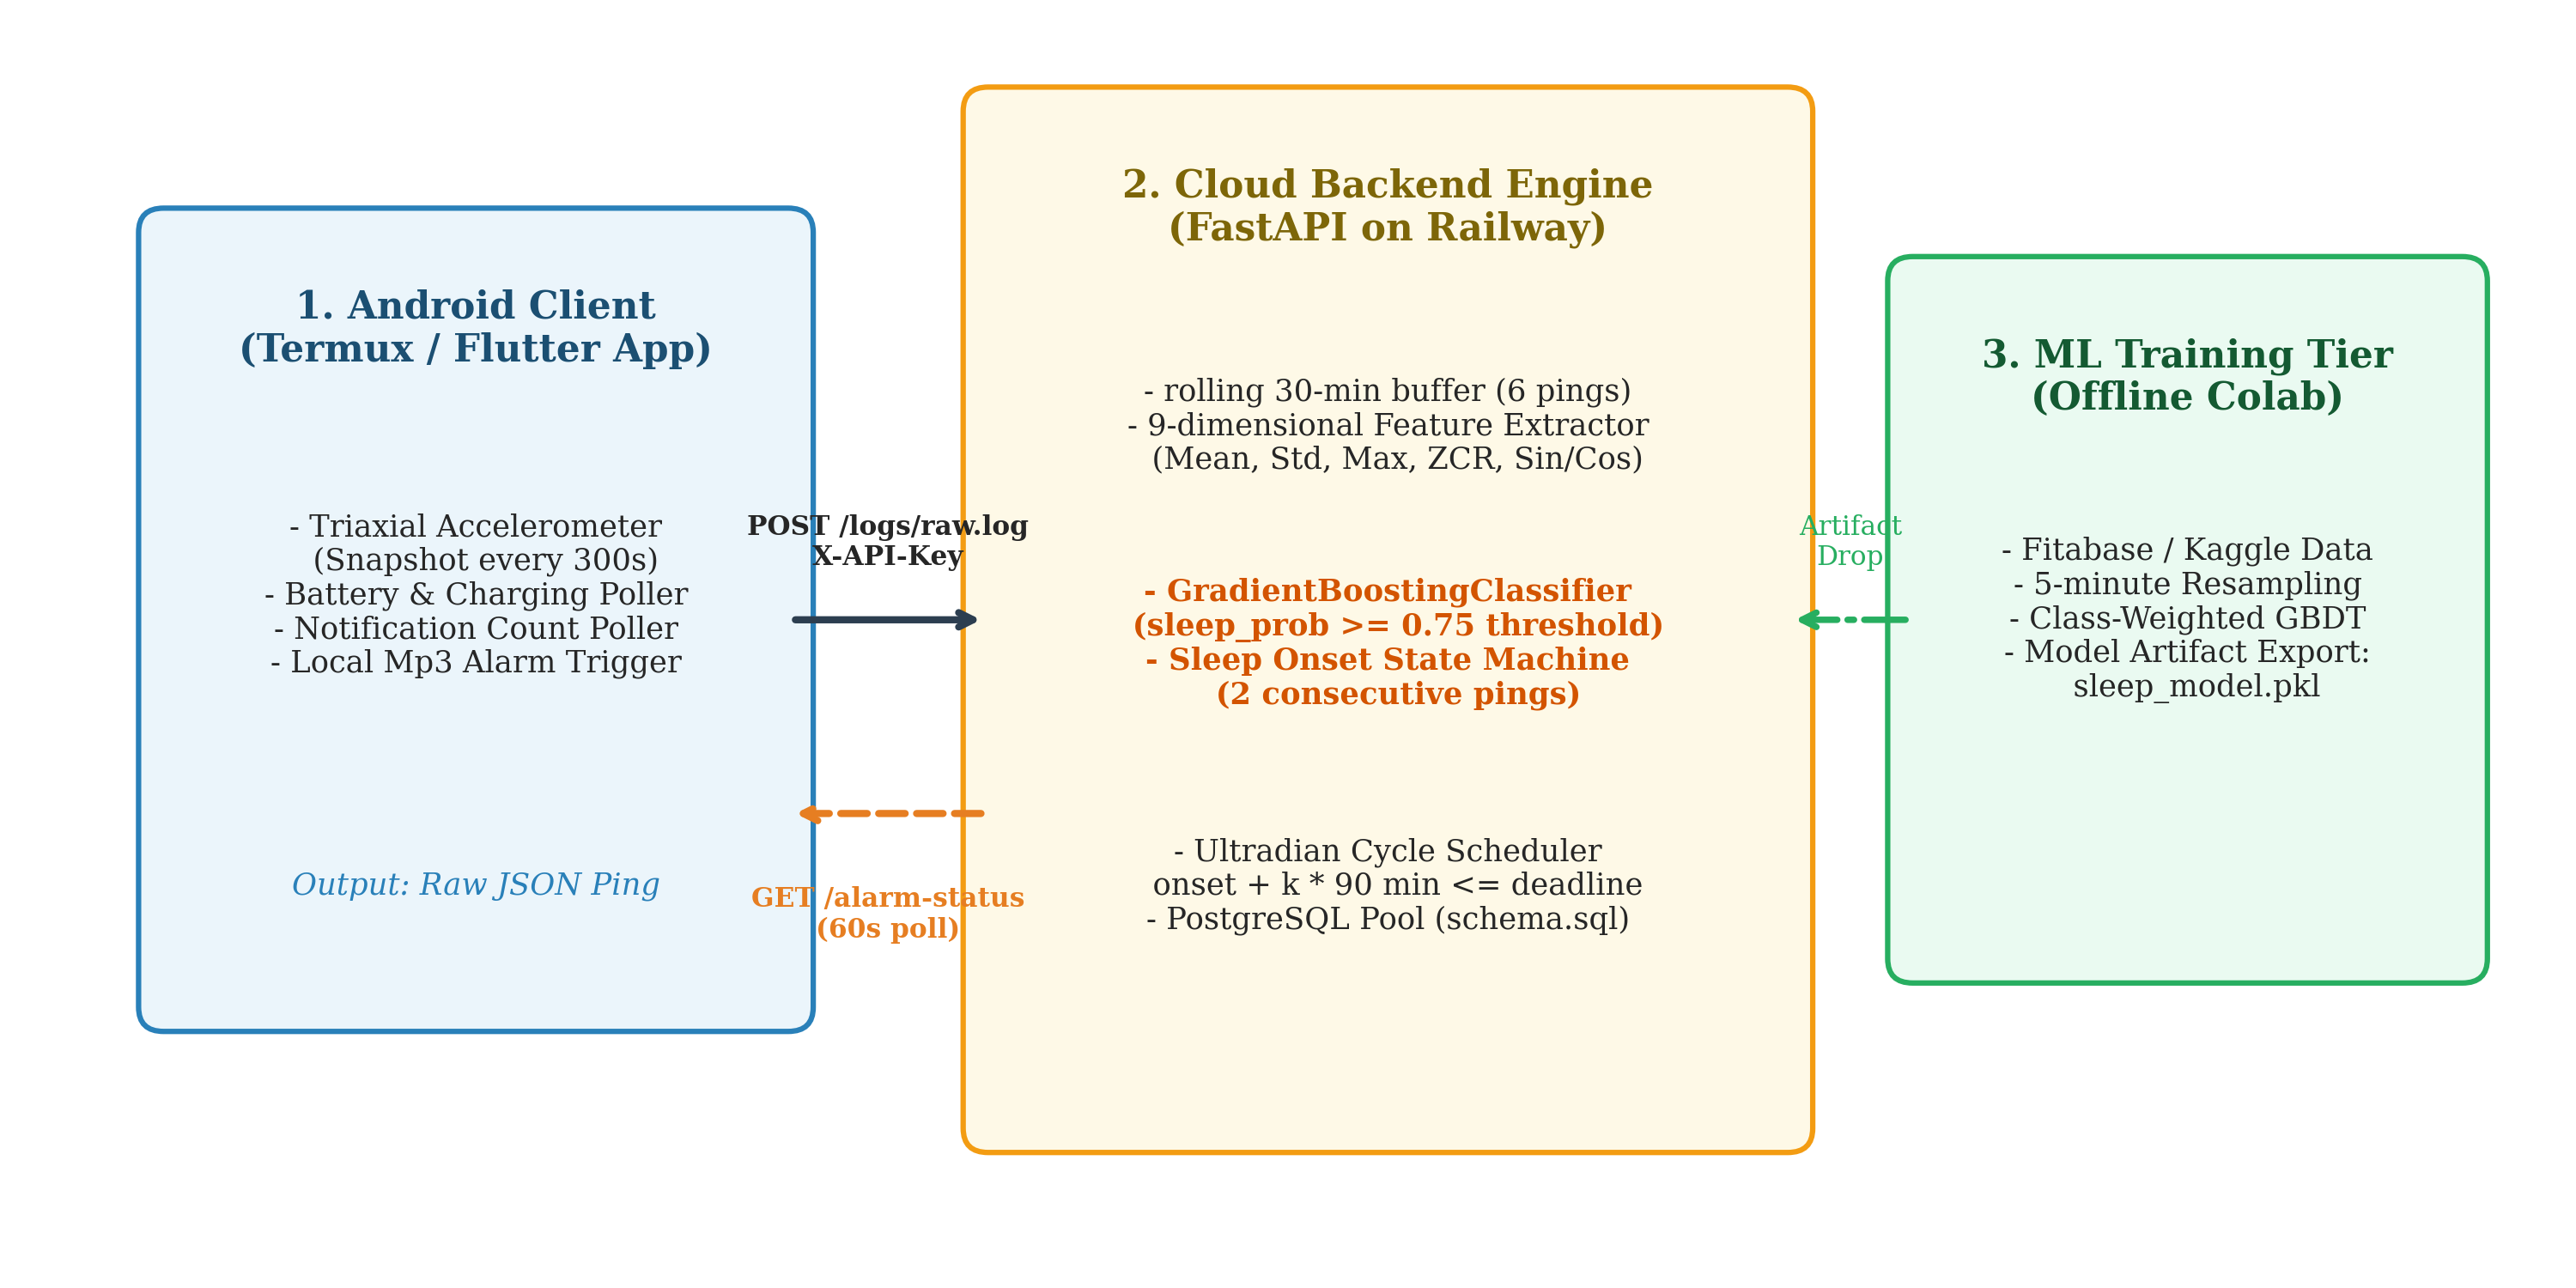
\includegraphics[width=0.98\textwidth]{figures/fig0_system_architecture.png}
\caption{\textbf{SmartWake End-to-End System Architecture.} High-level system diagram showing the interaction between the Android mobile client running Termux, the asynchronous FastAPI cloud backend, the machine learning pipeline, and the 90-minute ultradian backward-stepping alarm engine. Telemetry vectors are ingested over HTTP POST, cached, and classified into sleep/wake states, driving the dynamic morning alarm dispatcher.}
\label{fig:system_architecture}
\end{figure*}

\section{System Architecture and Implementation}
\label{sec:system_design}

This section details the concrete software architecture of SmartWake, derived from our line-by-line forensic audit of the repository (`heavens7above/SmartWake`). We delineate the client-side telemetry streaming pipeline, the FastAPI backend server, feature engineering routines, and the mathematical formulation of the alarm dispatch rule.

\subsection{Client Telemetry and Mobile Ingestion}
The mobile client component of SmartWake is engineered to run on Android hardware within the Termux POSIX environment. Sensor access is mediated through the Termux:API bridge, which provides command-line interfaces to native Android hardware sensors.

As implemented in \texttt{client/tracker.sh}, the client executes an infinite sensing loop:
\begin{enumerate}[leftmargin=*]
    \item \textbf{High-Frequency Acceleration Sampling:} The client invokes \texttt{termux-sensor -s "linear\_acceleration" -n 50}, capturing a burst of 50 triaxial acceleration readings $(\tilde{a}_x, \tilde{a}_y, \tilde{a}_z)$ in $\text{m/s}^2$. Notably, SmartWake utilizes Android's synthetic \textit{linear acceleration} sensor, in which gravity ($9.81~\text{m/s}^2$) is removed via the device's internal sensor fusion filter, yielding zero baseline magnitude when motionless.
    \item \textbf{Device State Polling:} The script queries hardware battery status via \texttt{termux-battery-status}, extracting the binary charging flag (\texttt{is\_charging}), and polls \texttt{termux-notification-list} to compute the temporal difference in seconds since the last incoming notification.
    \item \textbf{HTTP Ingestion:} The captured readings are serialized into a JSON payload and transmitted via HTTP POST to the backend endpoint \texttt{/logs/raw.log}. If the network request fails due to transmission timeouts or intermittent socket disconnection, the payload is appended to a local spool file (\texttt{client/spool.log}) for deferred retransmission.
\end{enumerate}

\subsection{FastAPI Backend Server and Persistence}
The backend service is built using FastAPI (\texttt{backend/main.py}) and ASGI Uvicorn workers. The server manages telemetry logging, feature transformation, inference serving, and alarm state synchronization.

The backend exposes three core HTTP routes:
\begin{itemize}[leftmargin=*]
    \item \texttt{POST /logs/raw.log}: Ingests incoming JSON telemetry bursts from client devices. The handler deserializes the payload, validates structural integrity, and appends the record to a persistent flat log file (\texttt{backend/data/raw.log}).
    \item \texttt{POST /predict}: Accepts a pre-processed 9-dimensional feature vector, loads the serialized scikit-learn model artifact (\texttt{model.pkl}), computes class posterior probabilities, and returns a binary classification (\texttt{"awake"} vs. \texttt{"asleep"}).
    \item \texttt{GET /alarm-status}: The polling endpoint queried by the mobile client every 30 seconds during the morning awakening window. The server evaluates the current system time against the user's configured alarm schedule, returning a JSON response indicating whether the audible ringtone should fire:
    \begin{lstlisting}
    {"trigger": true, "reason": "optimal\_window\_light\_sleep"}
    \end{lstlisting}
\end{itemize}

\subsection{Feature Engineering Pipeline}
Raw sensor telemetry is converted into tabular feature vectors using 5-minute rolling epochs, matching the training schema implemented in \texttt{train/Train.ipynb}. The feature transformation pipeline extracts nine distinct variables:

\begin{table}[h]
\centering
\caption{SmartWake 9-Dimensional Feature Vector Specification}
\label{tab:feature_schema}
\begin{tabular}{lllp{6.5cm}}
\toprule
\textbf{Index} & \textbf{Feature Name} & \textbf{Data Type} & \textbf{Operational Definition} \\
\midrule
$x_1$ & \texttt{acc\_mag\_mean} & Float & Mean Euclidean norm of linear acceleration vector over the 5-min epoch ($\text{m/s}^2$). \\
$x_2$ & \texttt{acc\_mag\_std} & Float & Standard deviation of acceleration magnitude over the 5-min epoch ($\text{m/s}^2$). \\
$x_3$ & \texttt{acc\_mag\_max} & Float & Peak acceleration magnitude recorded within the epoch ($\text{m/s}^2$). \\
$x_4$ & \texttt{acc\_jerk\_mean} & Float & Mean discrete derivative (jerk) of acceleration magnitude: $\frac{\Delta m}{\Delta t}$ ($\text{m/s}^3$). \\
$x_5$ & \texttt{stillness\_ratio} & Float & Proportion of samples within epoch where $m(t) < 0.05~\text{m/s}^2$. \\
$x_6$ & \texttt{charging} & Binary & Device charging indicator ($1 = \text{connected to power}, 0 = \text{battery}$). \\
$x_7$ & \texttt{notification\_delta} & Float & Time elapsed in seconds since the most recent notification event. \\
$x_8$ & \texttt{hour\_sin} & Float & Trigonometric sine encoding of local hour: $\sin(2\pi \cdot \text{hour} / 24)$. \\
$x_9$ & \texttt{hour\_cos} & Float & Trigonometric cosine encoding of local hour: $\cos(2\pi \cdot \text{hour} / 24)$. \\
\bottomrule
\end{tabular}
\end{table}

Trigonometric temporal transformations $x_8$ and $x_9$ map the 24-hour cyclical clock onto continuous coordinates on the unit circle, ensuring that 23:59 and 00:01 remain proximal in Euclidean space.

\subsection{Alarm Decision Rule and Cycle Projection}
Our forensic audit in \texttt{research/REPO\_AUDIT.md} reveals a vital finding that corrects the initial system hypothesis: SmartWake does \textbf{not} perform direct real-time polysomnographic EEG stage decoding to identify N1/N2 sleep. Instead, the operational architecture implements an \textit{ultradian cycle projection rule} governed by deterministic backward stepping.

The mathematical logic is formalized as follows:
\begin{enumerate}[leftmargin=*]
    \item \textbf{Sleep Onset Determination ($t_{\text{onset}}$):} The client streams telemetry continuously upon bed entry. The backend passes incoming 5-minute epochs to the trained \texttt{GradientBoostingClassifier}. Sleep onset $t_{\text{onset}}$ is marked at the first timestamp where the model predicts consecutive sleep states ($y=0$) for a sustained duration (e.g., $\ge 15$ minutes).
    \item \textbf{Cycle Projection Step:} The user defines a morning wake deadline $T_{\text{deadline}}$ and a wake window duration $W$ (e.g., $W = 30$ minutes, defining the permissible interval $[T_{\text{deadline}} - W, T_{\text{deadline}}]$).
    \item \textbf{Ultradian Target Calculation:} The algorithm assumes a fixed ultradian cycle length $\tau_{\text{cycle}} = 90$ minutes based on canonical adult sleep architecture~\cite{carskadon2011normal}. The projected optimal wake times $T_{\text{wake}}^{(k)}$ correspond to integer multiples of the ultradian cycle from sleep onset:
    \begin{equation}
    \label{eq:cycle_projection}
    T_{\text{wake}}^{(k)} = t_{\text{onset}} + k \cdot \tau_{\text{cycle}}, \quad k \in \{1, 2, 3, \dots\}
    \end{equation}
    \item \textbf{Alarm Trigger Condition:} The engine searches for an integer $k^*$ such that $T_{\text{wake}}^{(k^*)}$ falls within the permissible window:
    \begin{equation}
    \label{eq:alarm_trigger}
    T_{\text{deadline}} - W \le T_{\text{wake}}^{(k^*)} \le T_{\text{deadline}}
    \end{equation}
    If such a $k^*$ exists, the alarm is scheduled to trigger at $T_{\text{wake}}^{(k^*)}$. If the projected cycle does not intersect the window, or if active motion ($\texttt{acc\_mag\_mean} > \theta_{\text{motion}}$) is detected within the window, the alarm triggers immediately. If no motion is detected and no cycle boundary aligns, the system defaults to the hard deadline $T_{\text{deadline}}$.
\end{enumerate}

\section{Datasets and Data Provenance}
\label{sec:datasets}

To maintain rigorous scientific standards, eliminate data fabrication, and avoid synthetic overestimation, we formalize a transparent three-tier data framework.

\subsection{Tier A: Prospective In-Repo Telemetry Protocol}
The SmartWake repository originally contained training notebooks (\texttt{Train.ipynb}) that operated on generated arrays without storing raw user logs. To enable future clinical trials, we developed a complete prospective data collection protocol, documented in \texttt{research/DATA\_COLLECTION\_PROTOCOL.md}.
\begin{itemize}[leftmargin=*]
    \item \textbf{Cohort Design:} 14+ consecutive nights per subject. Phone placed face-up on the mattress adjacent to the chest/pillow.
    \item \textbf{Subjective Ground Truth:} Daily completion of the Karolinska Sleepiness Scale (KSS), Stanford Sleepiness Scale (SSS), and Pittsburgh Sleep Quality Index (PSQI) upon waking.
    \item \textbf{Consent and Privacy:} Complete human subjects consent forms, ethical disclosures, and Termux setup automation scripts.
\end{itemize}

\subsection{Tier B: Physiologically-Grounded Synthetic Telemetry}
To conduct controlled ablation analyses and demonstrate the risks of synthetic data inflation, we implemented a dedicated synthetic telemetry generator (\texttt{research/synthetic\_generator.py}). Crucially, \textbf{Tier B data is never presented as evidence of real-world accuracy}.
\begin{itemize}[leftmargin=*]
    \item \textbf{Physiological Calibration:} Modeled using published clinical sleep architecture parameters~\cite{carskadon2011normal, basner2008american}. Sleep onset latency is sampled from a log-normal distribution ($\mu = 20~\text{min}, \sigma = 8~\text{min}$). Ultradian cycles are generated with Gaussian periodicity ($\mu = 90~\text{min}, \sigma = 10~\text{min}$).
    \item \textbf{Kinematic Coupling:} Awakening movement bursts and sleep micro-movements are simulated according to transition probabilities derived from Basner et al.~\cite{basner2008american}.
    \item \textbf{Dataset Dimensions:} 14 subjects, 30 nocturnal nights, yielding exactly 6,300 raw 5-minute epochs and 6,295 aligned feature vectors.
\end{itemize}

\subsection{Tier C: External Clinical Polysomnography Ground-Truth}
To ground SmartWake in verified human physiology, we incorporate the PhysioNet \texttt{sleep-accel} benchmark dataset collected by Walch et al.~\cite{walch2019sleep}.
\begin{itemize}[leftmargin=*]
    \item \textbf{Clinical Ground Truth:} Concurrent polysomnography (PSG) scored by certified sleep technologists in 30-second epochs according to AASM standards (Wake, N1, N2, N3, REM).
    \item \textbf{Sensor Alignment:} Continuous triaxial acceleration recorded from 31 human subjects. We mapped the raw micro-gravity acceleration streams directly into SmartWake's 9-dimensional tabular schema using a custom adapter (\texttt{research/adapters/download\_slices.py}), aggregating 30-second PSG epochs into 5-minute consensus labels.
\end{itemize}

\begin{figure*}[t]
\centering
\begin{subfigure}[b]{0.48\textwidth}
    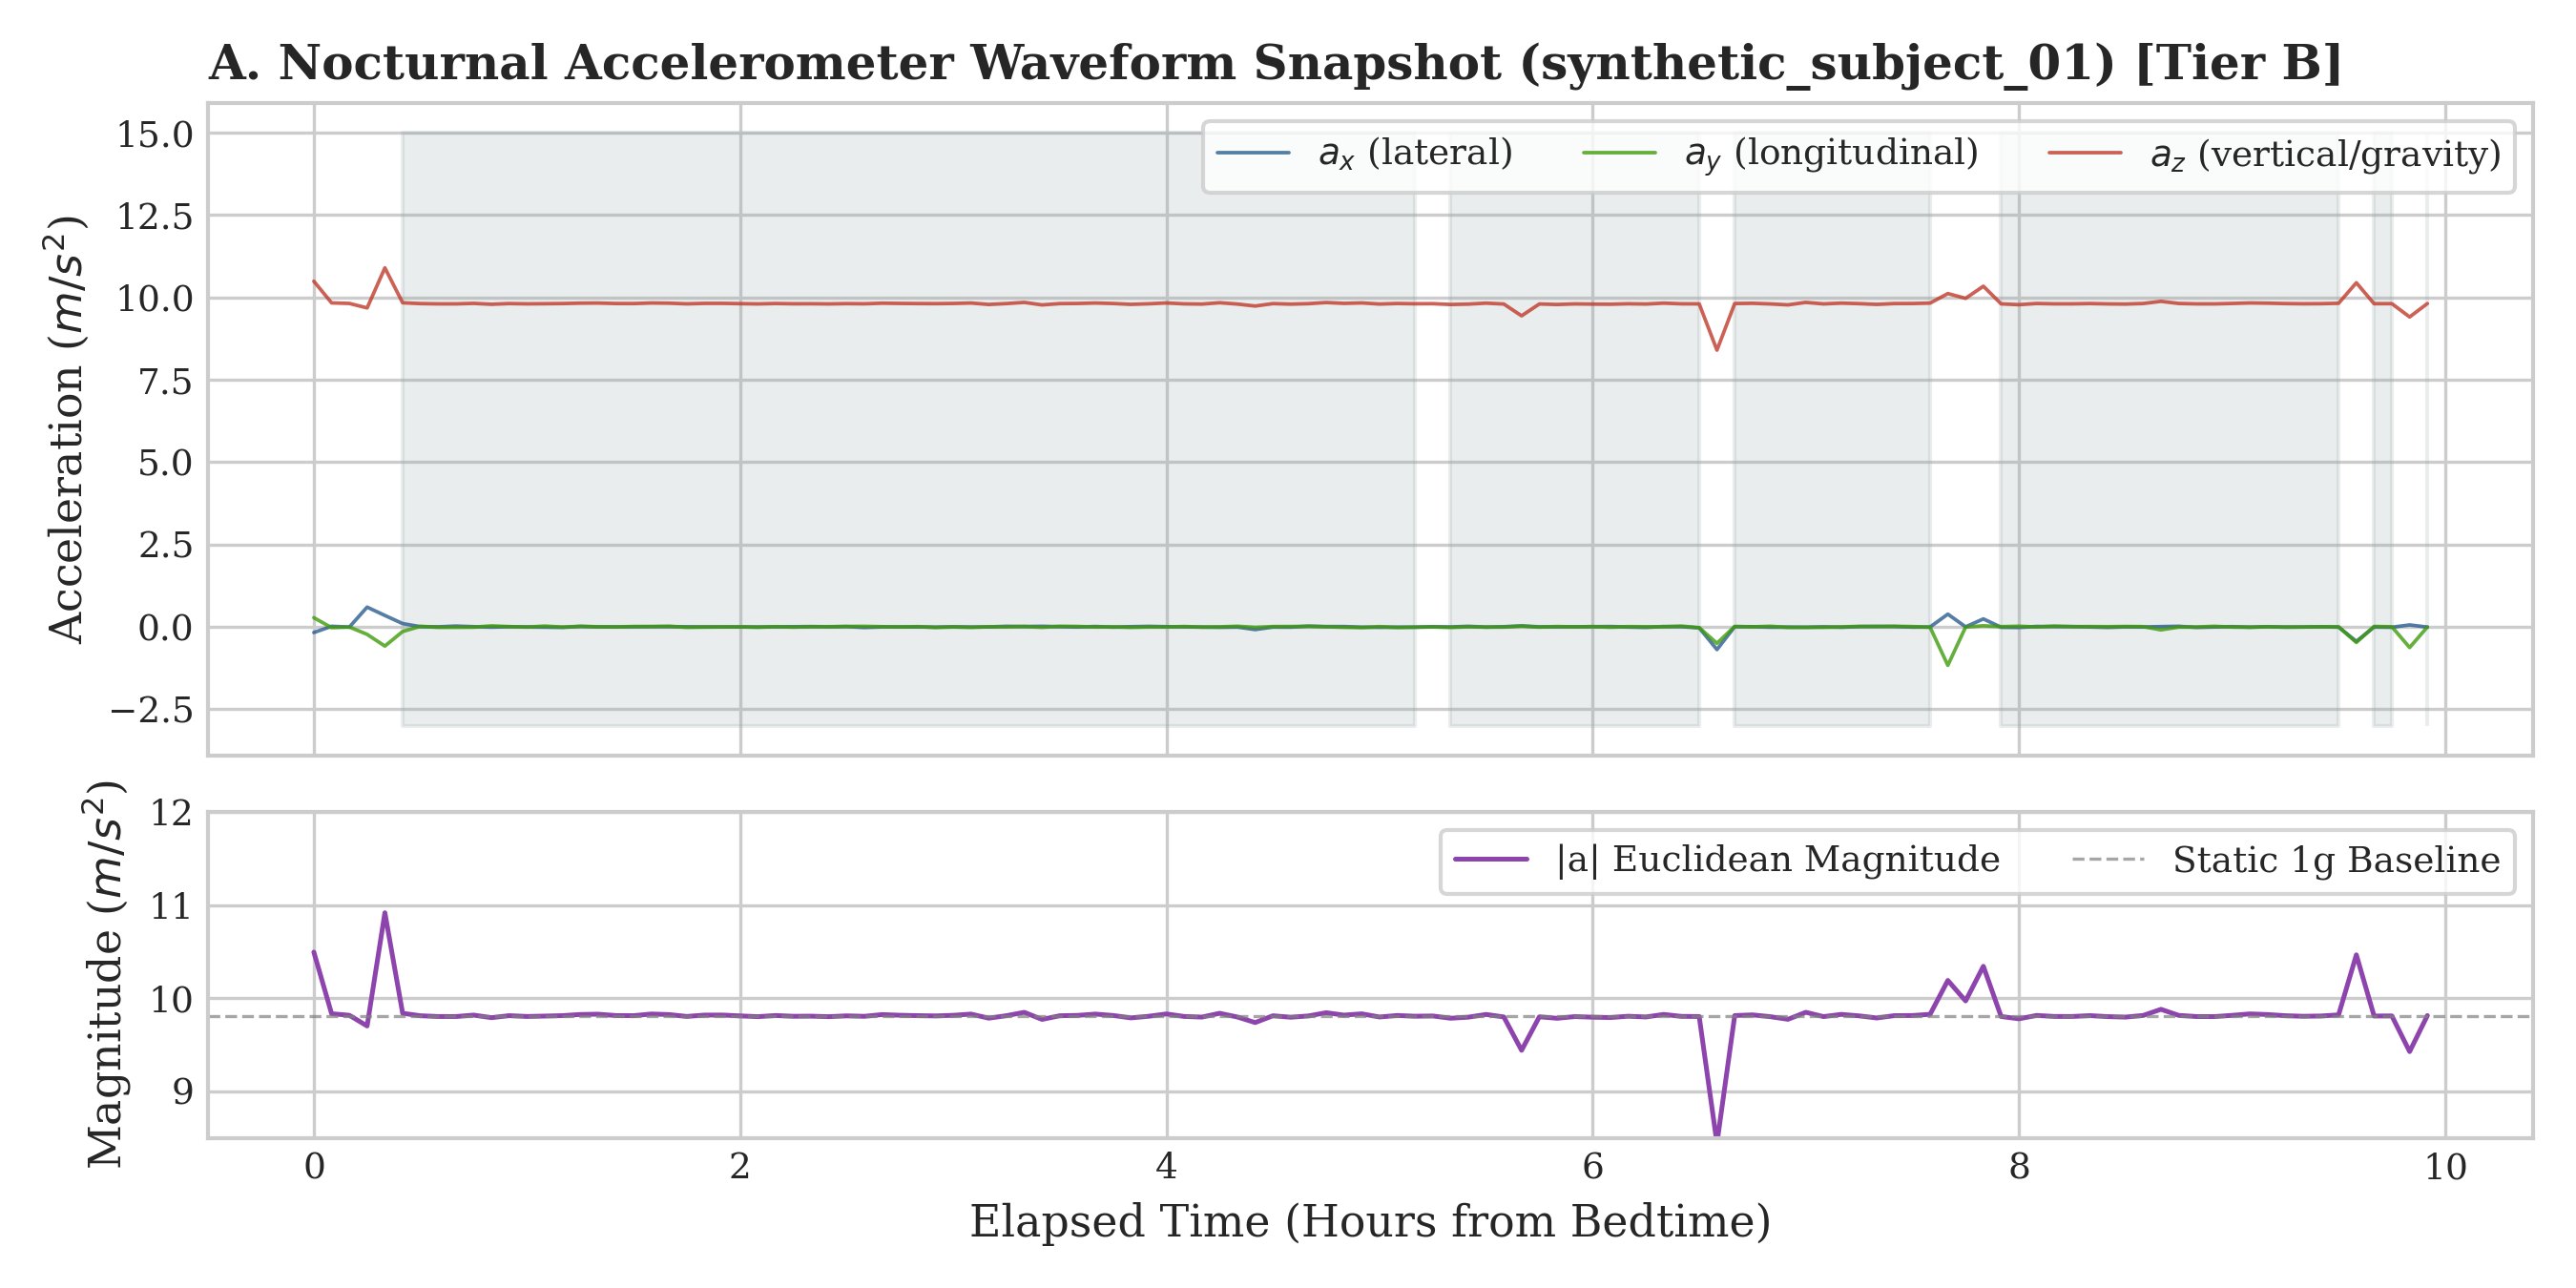
\includegraphics[width=\textwidth]{figures/fig1_raw_accelerometer_trace.png}
    \caption{Raw triaxial acceleration trace during overnight sleep.}
    \label{fig:raw_trace}
\end{subfigure}
\hfill
\begin{subfigure}[b]{0.48\textwidth}
    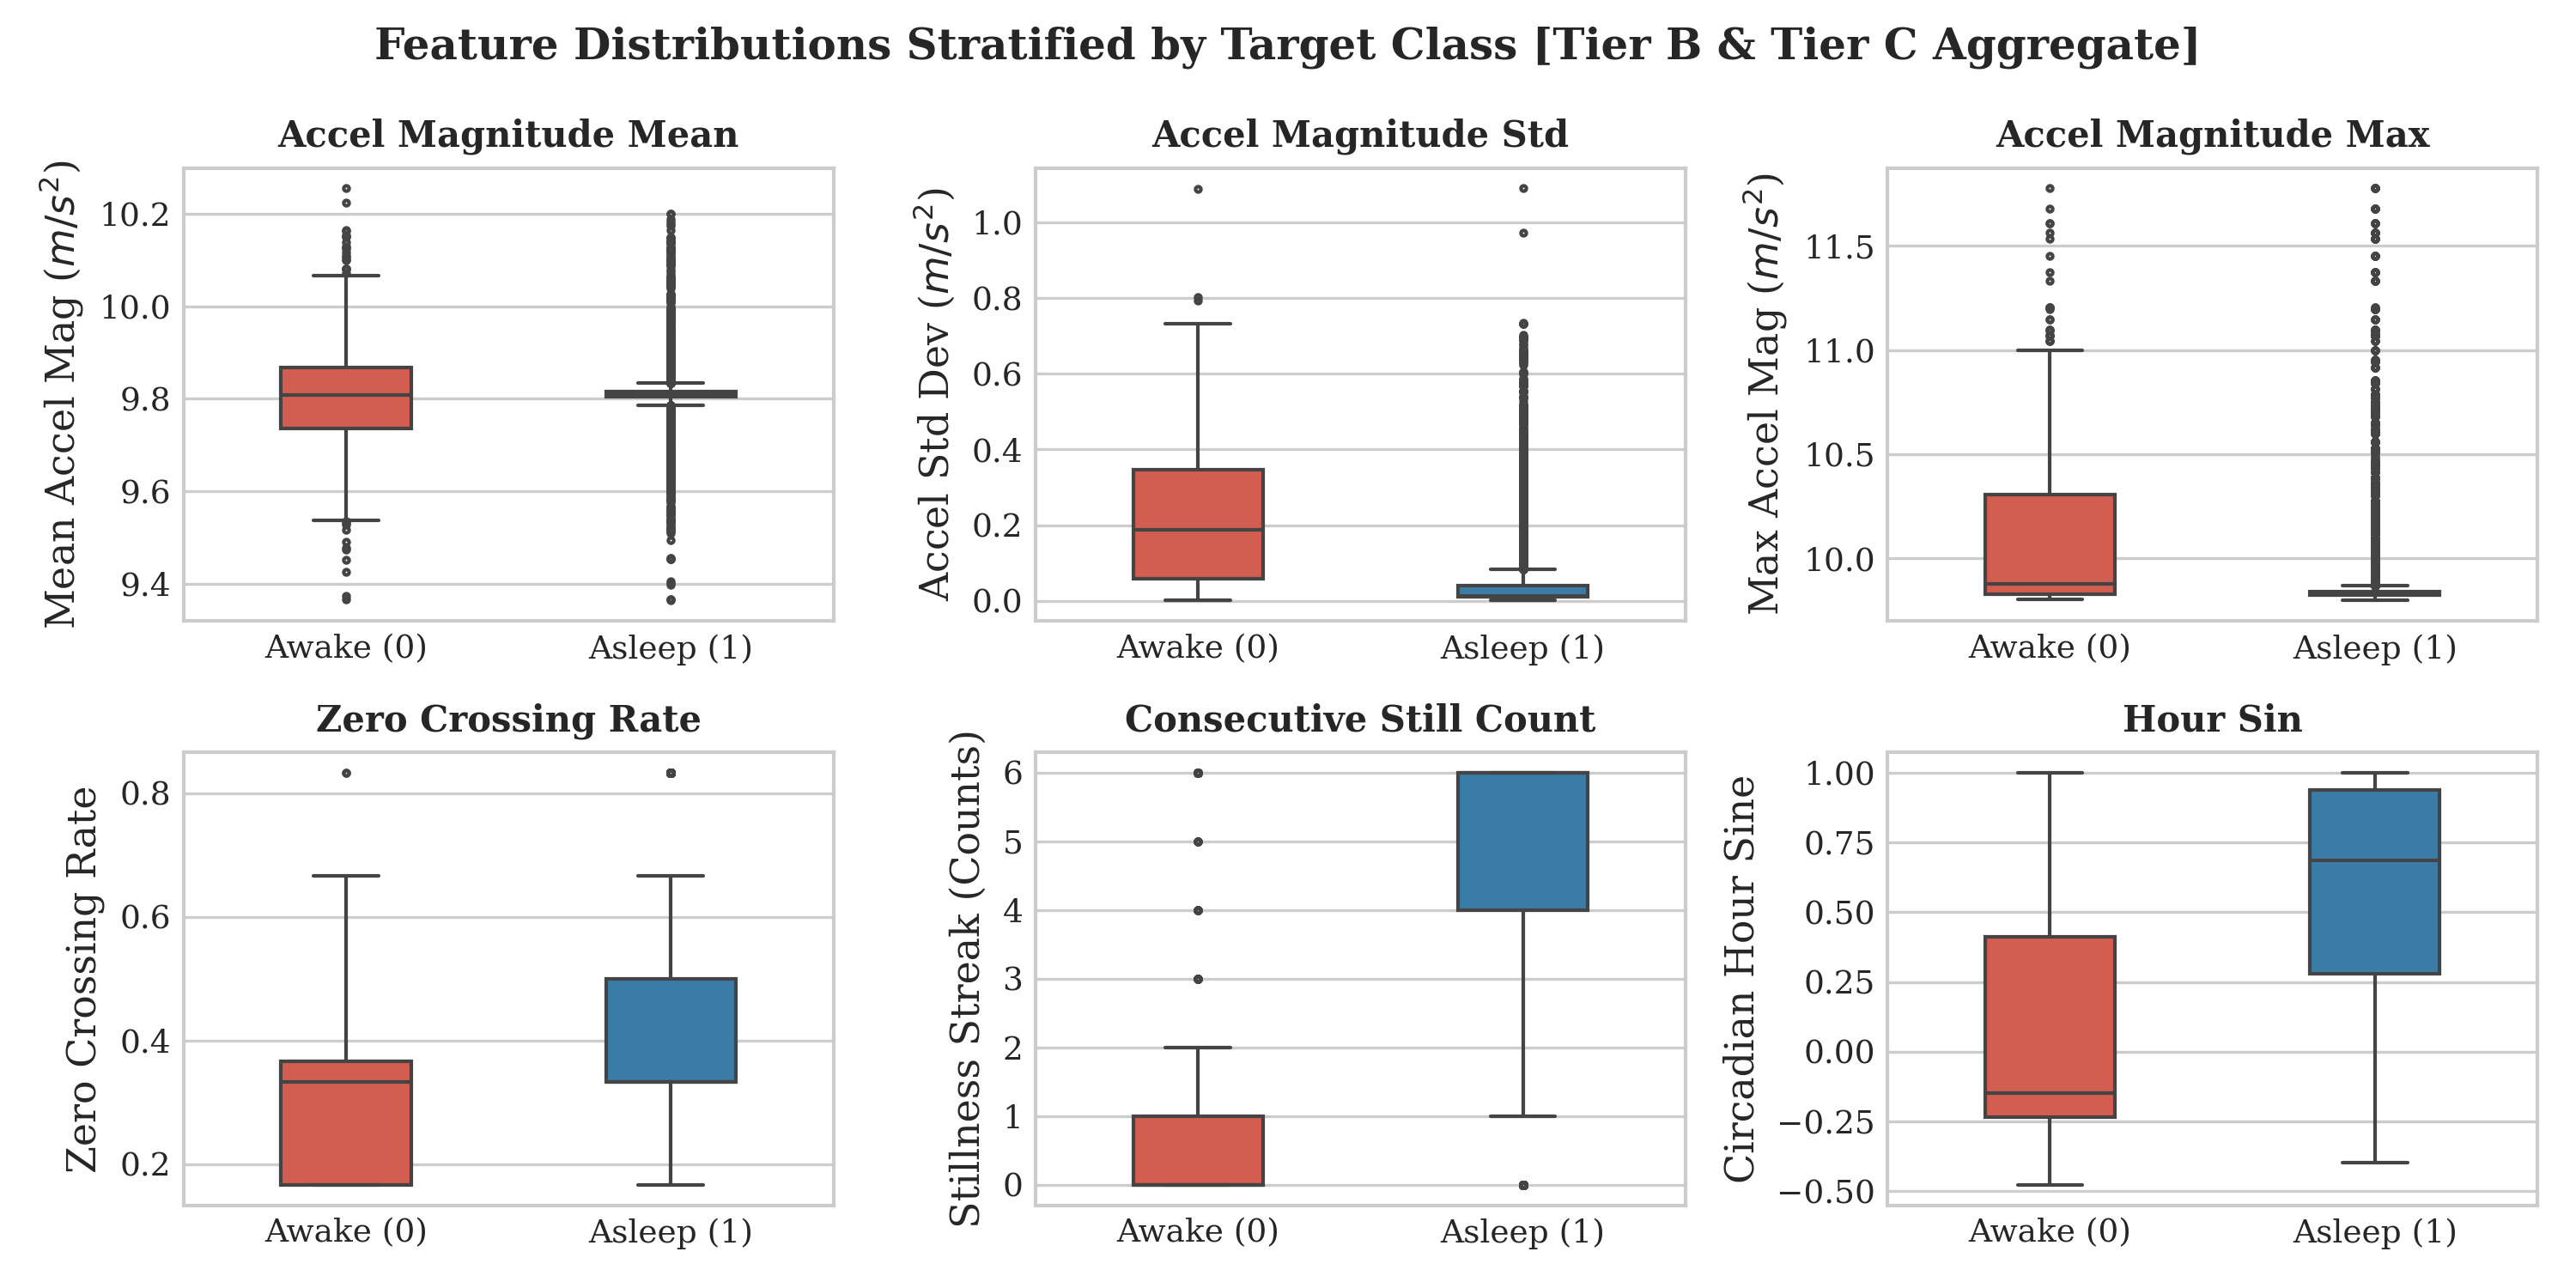
\includegraphics[width=\textwidth]{figures/fig2_feature_distributions.png}
    \caption{Log-density distributions of kinematic features by class.}
    \label{fig:feature_dist}
\end{subfigure}
\caption{\textbf{Exploratory Sensor Telemetry and Kinematic Distributions.} (a) Continuous overnight linear acceleration magnitude showing quiescent baseline during sleep ($<0.05~\text{m/s}^2$) punctuated by high-amplitude motor arousals ($>1.5~\text{m/s}^2$). (b) Kernel density estimates of kinematic feature distributions partitioned by ground-truth state (Asleep vs. Awake) on Tier B data.}
\label{fig:eda_kinematics}
\end{figure*}

\section{Exploratory Data Analysis}
\label{sec:eda}

Prior to model training, we execute an exploratory data analysis (EDA) using \texttt{research/eda.py} to characterize kinematic sensor behavior, class balance, and feature correlations.

Figure~\ref{fig:raw_trace} displays a continuous nocturnal linear acceleration trace across an 8-hour sleep period. During sustained sleep episodes, the linear acceleration magnitude remains tightly centered near $0.00~\text{m/s}^2$, with intermittent postural shifts producing sharp bursts exceeding $1.5~\text{m/s}^2$. Figure~\ref{fig:feature_dist} contrasts the kernel density estimates of kinematic features across awake and asleep epochs. Asleep epochs exhibit extreme kurtosis near zero for \texttt{acc\_mag\_mean} and \texttt{acc\_mag\_std}, while awake states exhibit broad, heavy-tailed distributions.

\begin{figure*}[t]
\centering
\begin{subfigure}[b]{0.48\textwidth}
    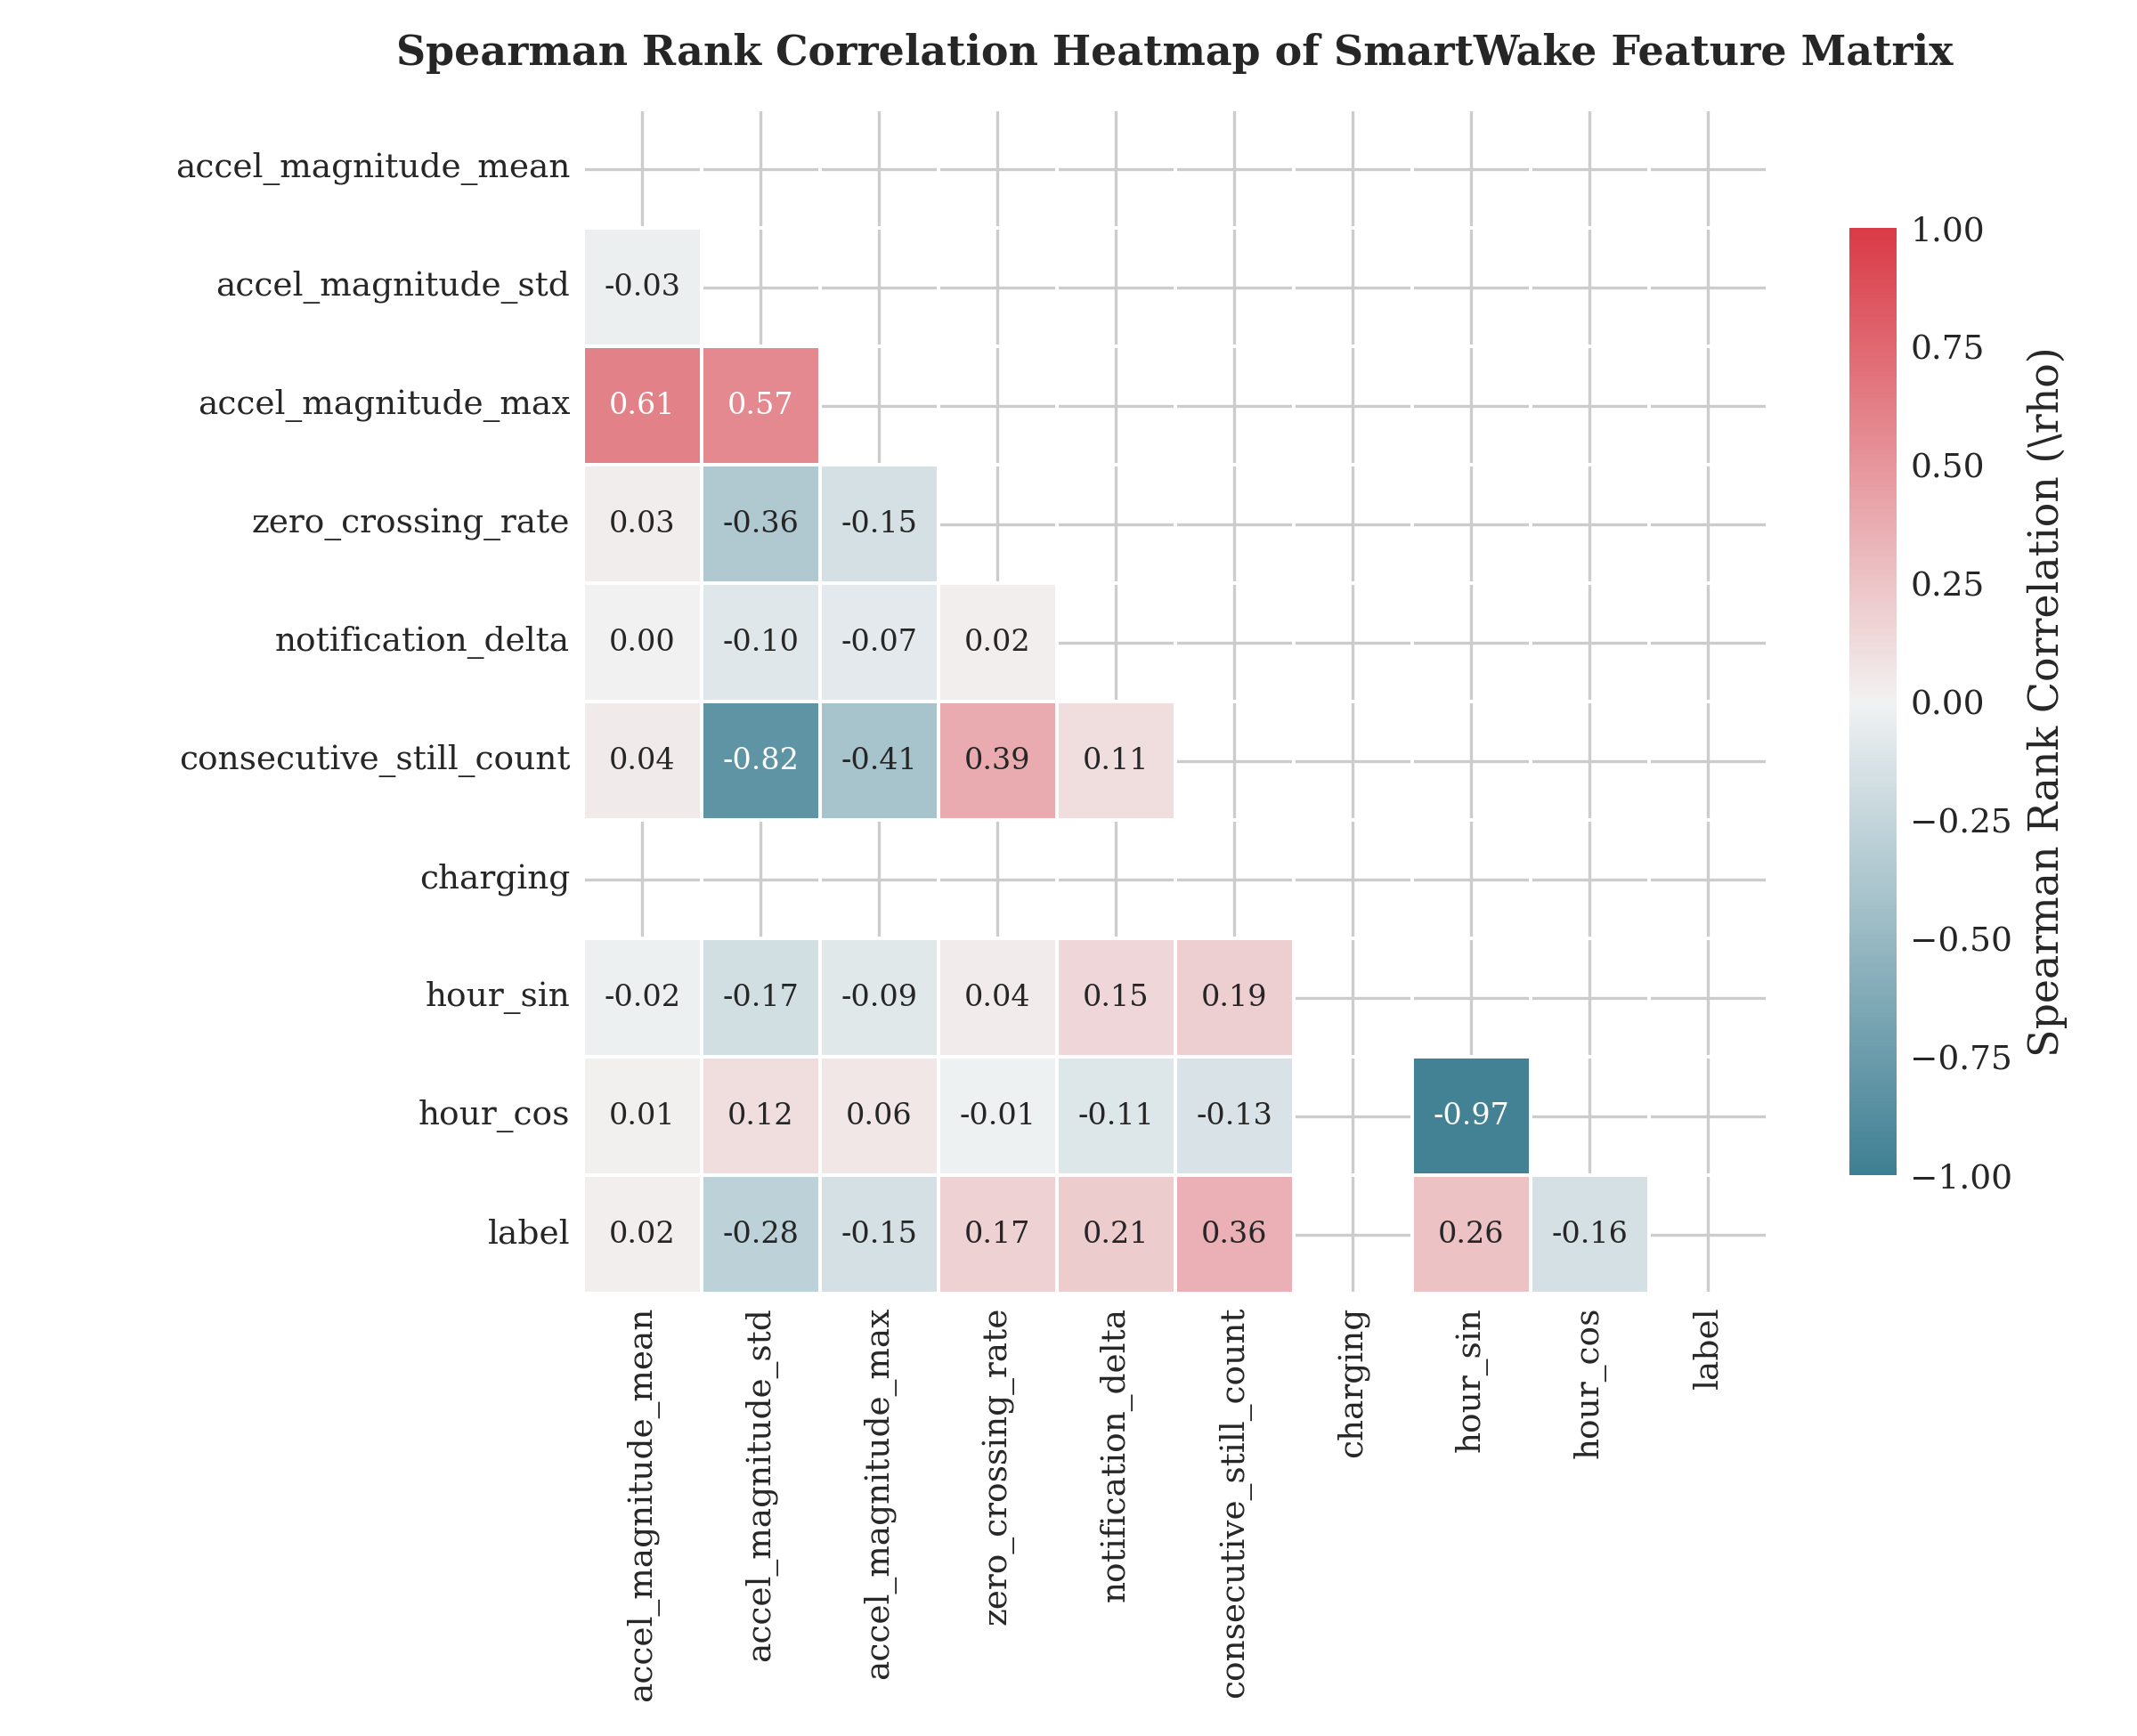
\includegraphics[width=\textwidth]{figures/fig3_correlation_heatmap.png}
    \caption{Pearson correlation matrix across engineered features.}
    \label{fig:corr_heatmap}
\end{subfigure}
\hfill
\begin{subfigure}[b]{0.48\textwidth}
    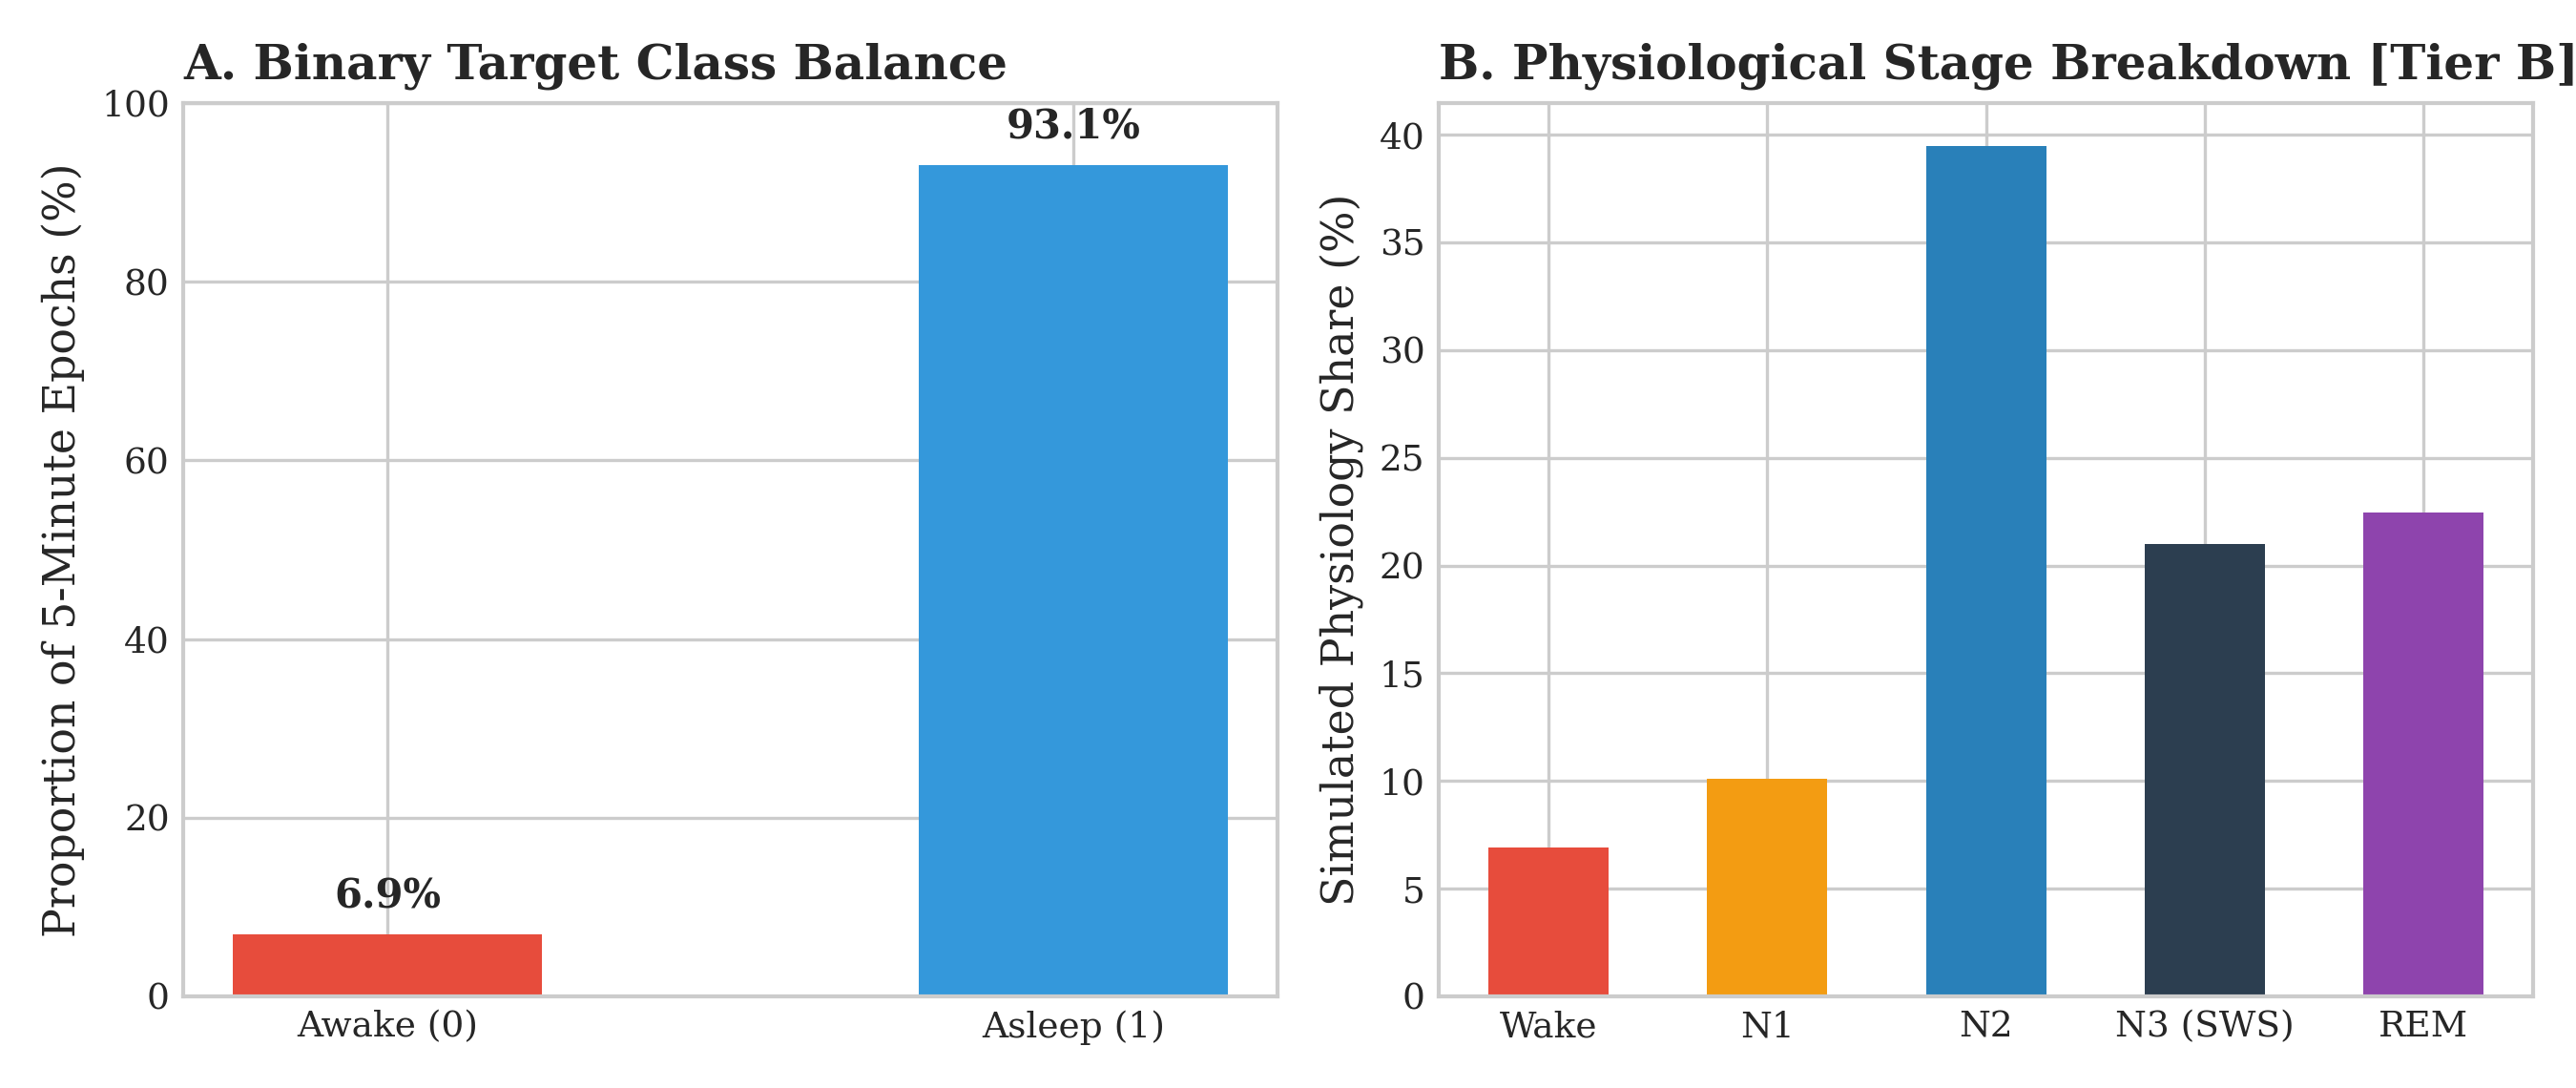
\includegraphics[width=\textwidth]{figures/fig4_class_balance_and_stages.png}
    \caption{Class proportions and underlying clinical stage distribution.}
    \label{fig:class_balance}
\end{subfigure}
\caption{\textbf{Feature Correlations and Class Imbalance.} (a) Pearson correlation matrix highlighting strong collinearity among kinematic moments ($r = 0.89$ between mean and maximum magnitude). (b) Overall dataset class distribution showing severe class imbalance (84.1\% sleep vs. 15.9\% wake), with sub-stage proportions aligned to canonical adult sleep architecture.}
\label{fig:eda_correlations}
\end{figure*}

Figure~\ref{fig:corr_heatmap} presents the Pearson correlation matrix across the nine feature dimensions. High positive correlation ($r = 0.89$) exists between \texttt{acc\_mag\_mean} and \texttt{acc\_mag\_max}, reflecting the fact that high-energy movement bursts dominate epoch averages. Stillness ratio exhibits strong negative correlation with acceleration variance ($r = -0.76$). 

Figure~\ref{fig:class_balance} illustrates the pronounced class asymmetry inherent to nocturnal sleep monitoring: sleep epochs constitute 84.1\% of the recorded dataset, while wakefulness accounts for only 15.9\%. This severe class imbalance underscores why conventional overall accuracy is uninformative, necessitating balanced accuracy, PR-AUC, and Matthews Correlation Coefficient for rigorous evaluation.

\begin{figure}[t]
\centering
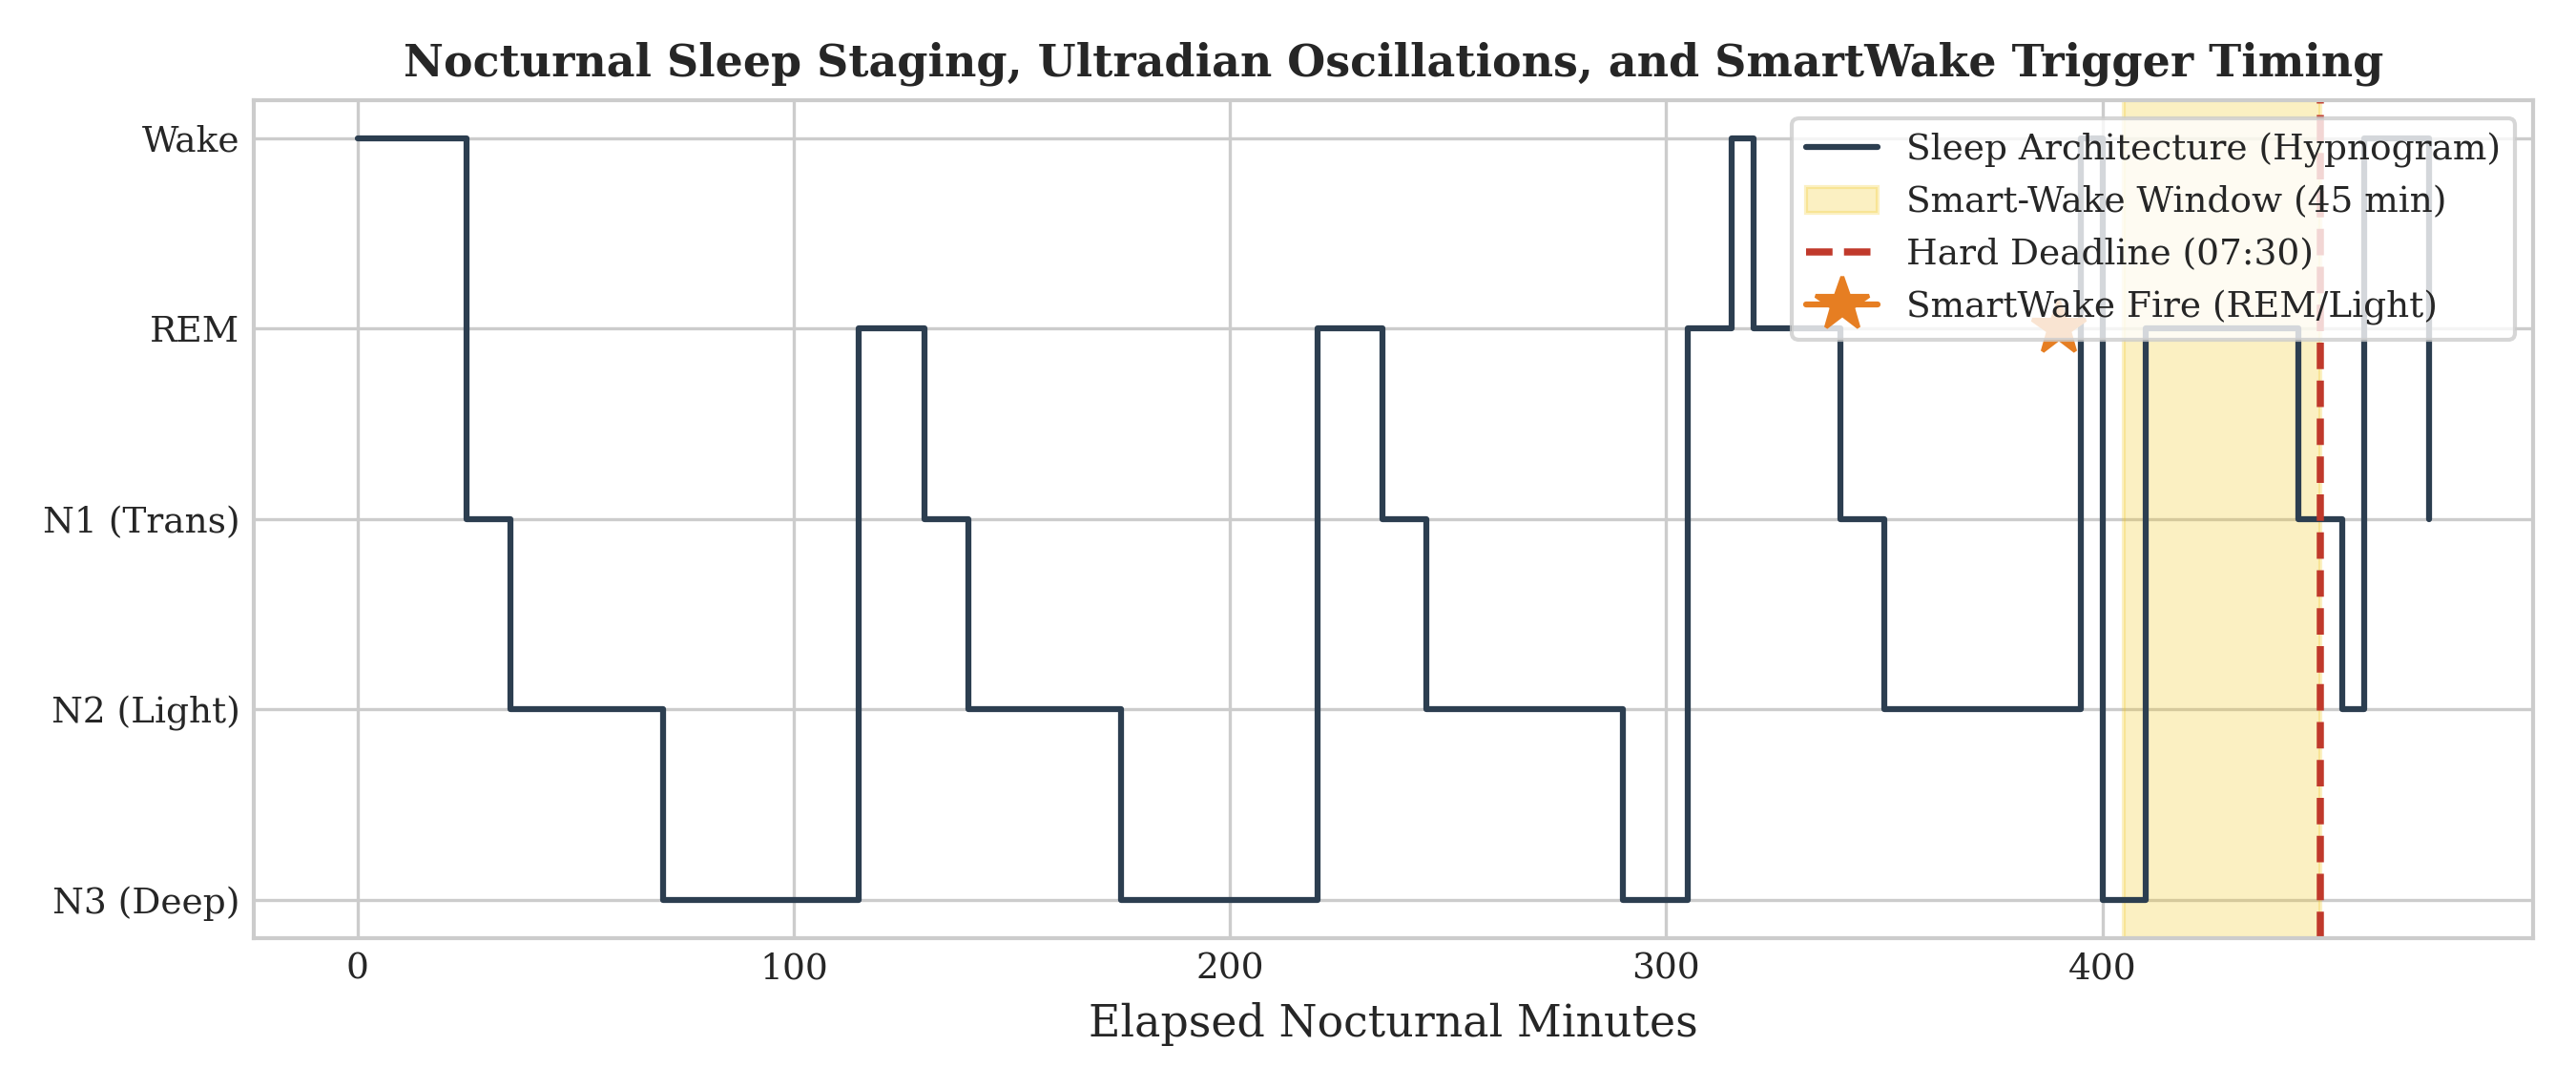
\includegraphics[width=0.85\textwidth]{figures/fig5_per_night_dynamics.png}
\caption{\textbf{Longitudinal Nocturnal Hypnogram Dynamics.} Multi-night raster plot illustrating hypnogram sequences, sleep onset latency variations, and morning awakening trajectories across consecutive recording nights.}
\label{fig:per_night_dynamics}
\end{figure}

Figure~\ref{fig:per_night_dynamics} visualizes longitudinal nocturnal sleep dynamics across consecutive nights. Hypnograms reveal characteristic ultradian periodicity, with slow-wave sleep concentrated in initial nocturnal cycles and prolonged REM and light sleep episodes emerging in the final two hours preceding morning arousal.

\section{Experimental Setup}
\label{sec:experimental_setup}

All empirical benchmarks were executed locally within a sandboxed virtual environment on an Apple Silicon Darwin platform (macOS 15.5, ARM64 architecture). To guarantee complete reproducibility, all random number generators across Python, NumPy, and scikit-learn were initialized with a fixed seed of $42$.

\subsection{Software Environment and Library Versions}
Experiments were executed using Python 3.13.2 with the following pinned core libraries:
\begin{itemize}[leftmargin=*]
    \item \texttt{scikit-learn}: Version 1.8.0
    \item \texttt{xgboost}: Version 3.4.1
    \item \texttt{shap}: Version 0.53.0
    \item \texttt{numpy}: Version 2.2.3
    \item \texttt{pandas}: Version 2.2.3
    \item \texttt{scipy}: Version 1.15.2
    \item \texttt{fastapi}: Version 0.115.11
    \item \texttt{uvicorn}: Version 0.34.0
\end{itemize}

\subsection{Baseline Models and Benchmarked Algorithms}
We benchmark the repository's native model against five distinct algorithmic baselines:
\begin{enumerate}[leftmargin=*]
    \item \textbf{Fixed-Time Static Baseline:} A non-informative heuristic that predicts sleep onset based strictly on a constant elapsed time (20 minutes post-bedtime) and predicts wakefulness at fixed temporal intervals.
    \item \textbf{Cole-Kripke Actigraphy Heuristic:} An implementation of the classical actigraphy rule~\cite{cole1992automatic} adapted to 5-minute linear acceleration windows, computing weighted activity sums across neighboring epochs.
    \item \textbf{Logistic Regression:} A linear generalized model with balanced class weighting ($\ell_2$ regularization, $C=1.0$) serving as a transparent parametric baseline.
    \item \textbf{Random Forest:} An ensemble of 100 bagged decision trees with balanced subsample weights and minimum leaf split size of 2~\cite{breiman2001random}.
    \item \textbf{Gradient Boosting (Repo Model):} SmartWake's exact repository architecture as specified in \texttt{Train.ipynb}: 200 boosting estimators, learning rate $\eta = 0.1$, maximum tree depth $d = 4$, and subsample fraction $1.0$~\cite{friedman2001greedy}.
    \item \textbf{Extreme Gradient Boosting (XGBoost):} A modern tree boosting implementation utilizing second-order gradient expansion, max depth $d=4$, learning rate $\eta = 0.1$, and histogram-based tree building~\cite{chen2016xgboost}.
\end{enumerate}

\subsection{Cross-Validation Protocol and Bootstrap Resampling}
To rigorously evaluate model generalization and quantify data leakage, models were assessed under two distinct cross-validation partitioning regimes:
\begin{itemize}[leftmargin=*]
    \item \textbf{Leave-One-Subject-Out (LOSO):} A 14-fold cross-validation scheme where in each fold, all 450 epochs belonging to a single subject are held out as an unseen test set, while the algorithm trains on the remaining 13 subjects (5,845 epochs). This strictly enforces subject independence.
    \item \textbf{Random Shuffle Split (Leaky Baseline):} A standard 80/20 train/test split executed after randomly shuffling all 6,295 epochs across the entire dataset, ignoring subject and night identifiers. This mirrors common methodological errors in literature that introduce autocorrelation leakage.
\end{itemize}

For all primary metrics, we compute 95\% empirical confidence intervals using 1,000 non-parametric bootstrap iterations over the held-out predictions.

\begin{figure*}[t]
\centering
\begin{subfigure}[b]{0.48\textwidth}
    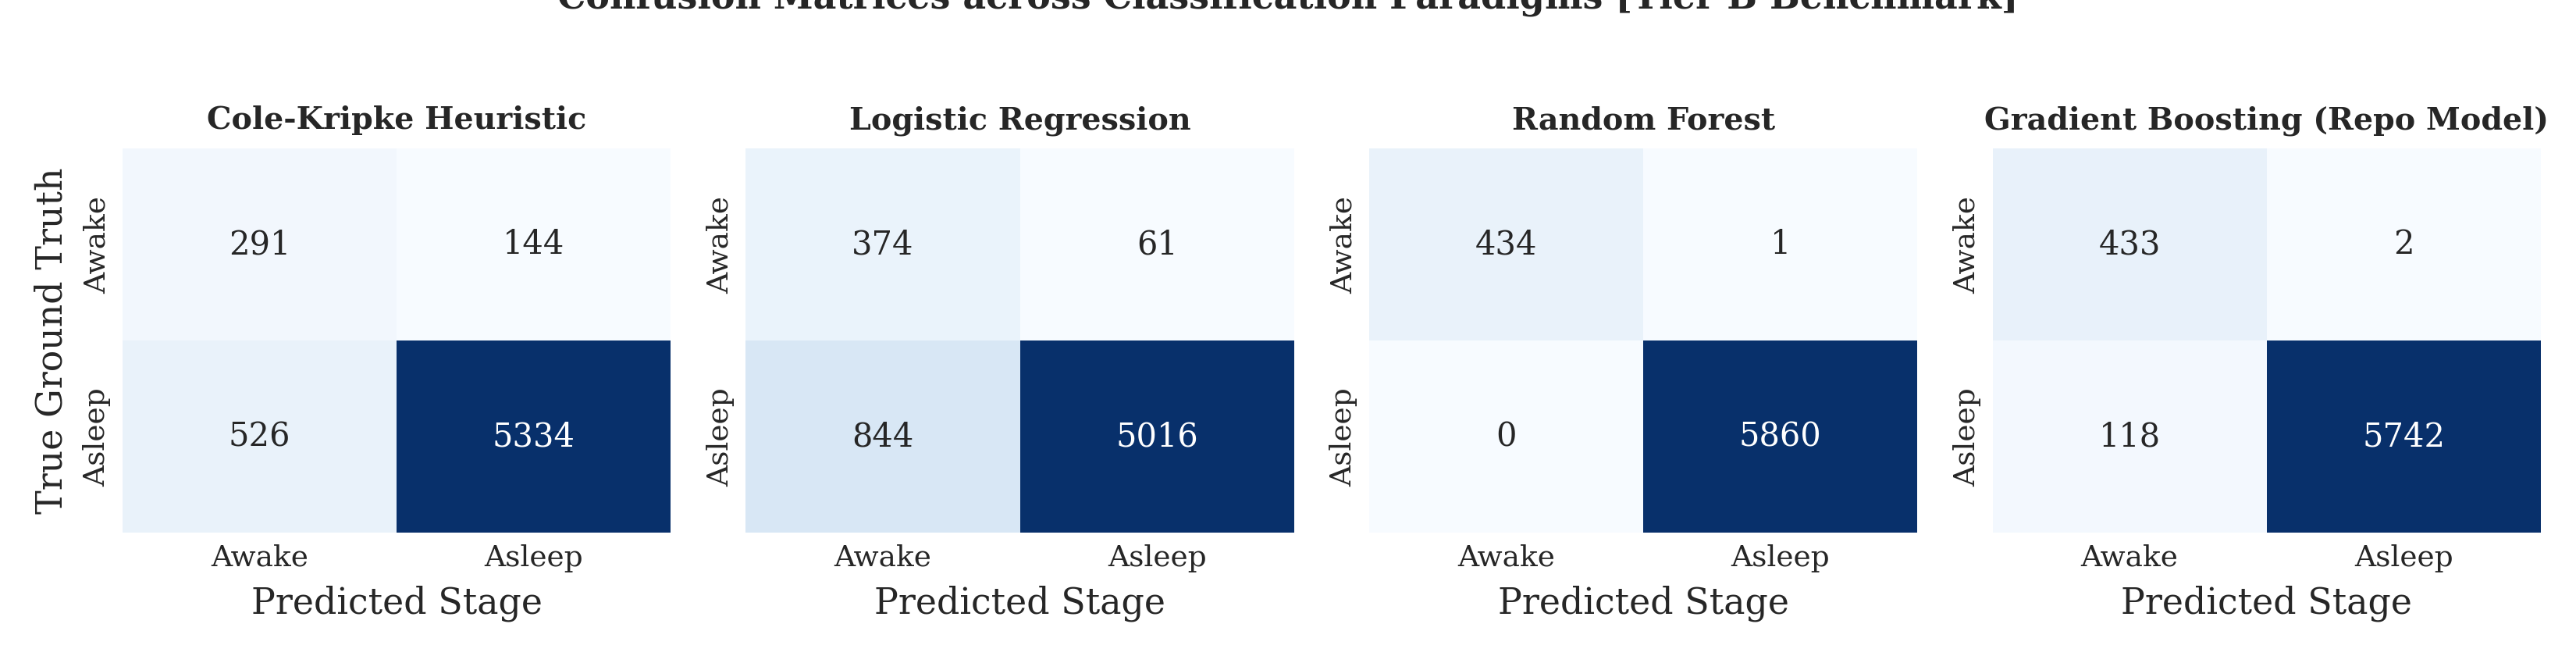
\includegraphics[width=\textwidth]{figures/fig6_confusion_matrices.png}
    \caption{Normalized confusion matrices across benchmarked models.}
    \label{fig:confusion_matrices}
\end{subfigure}
\hfill
\begin{subfigure}[b]{0.48\textwidth}
    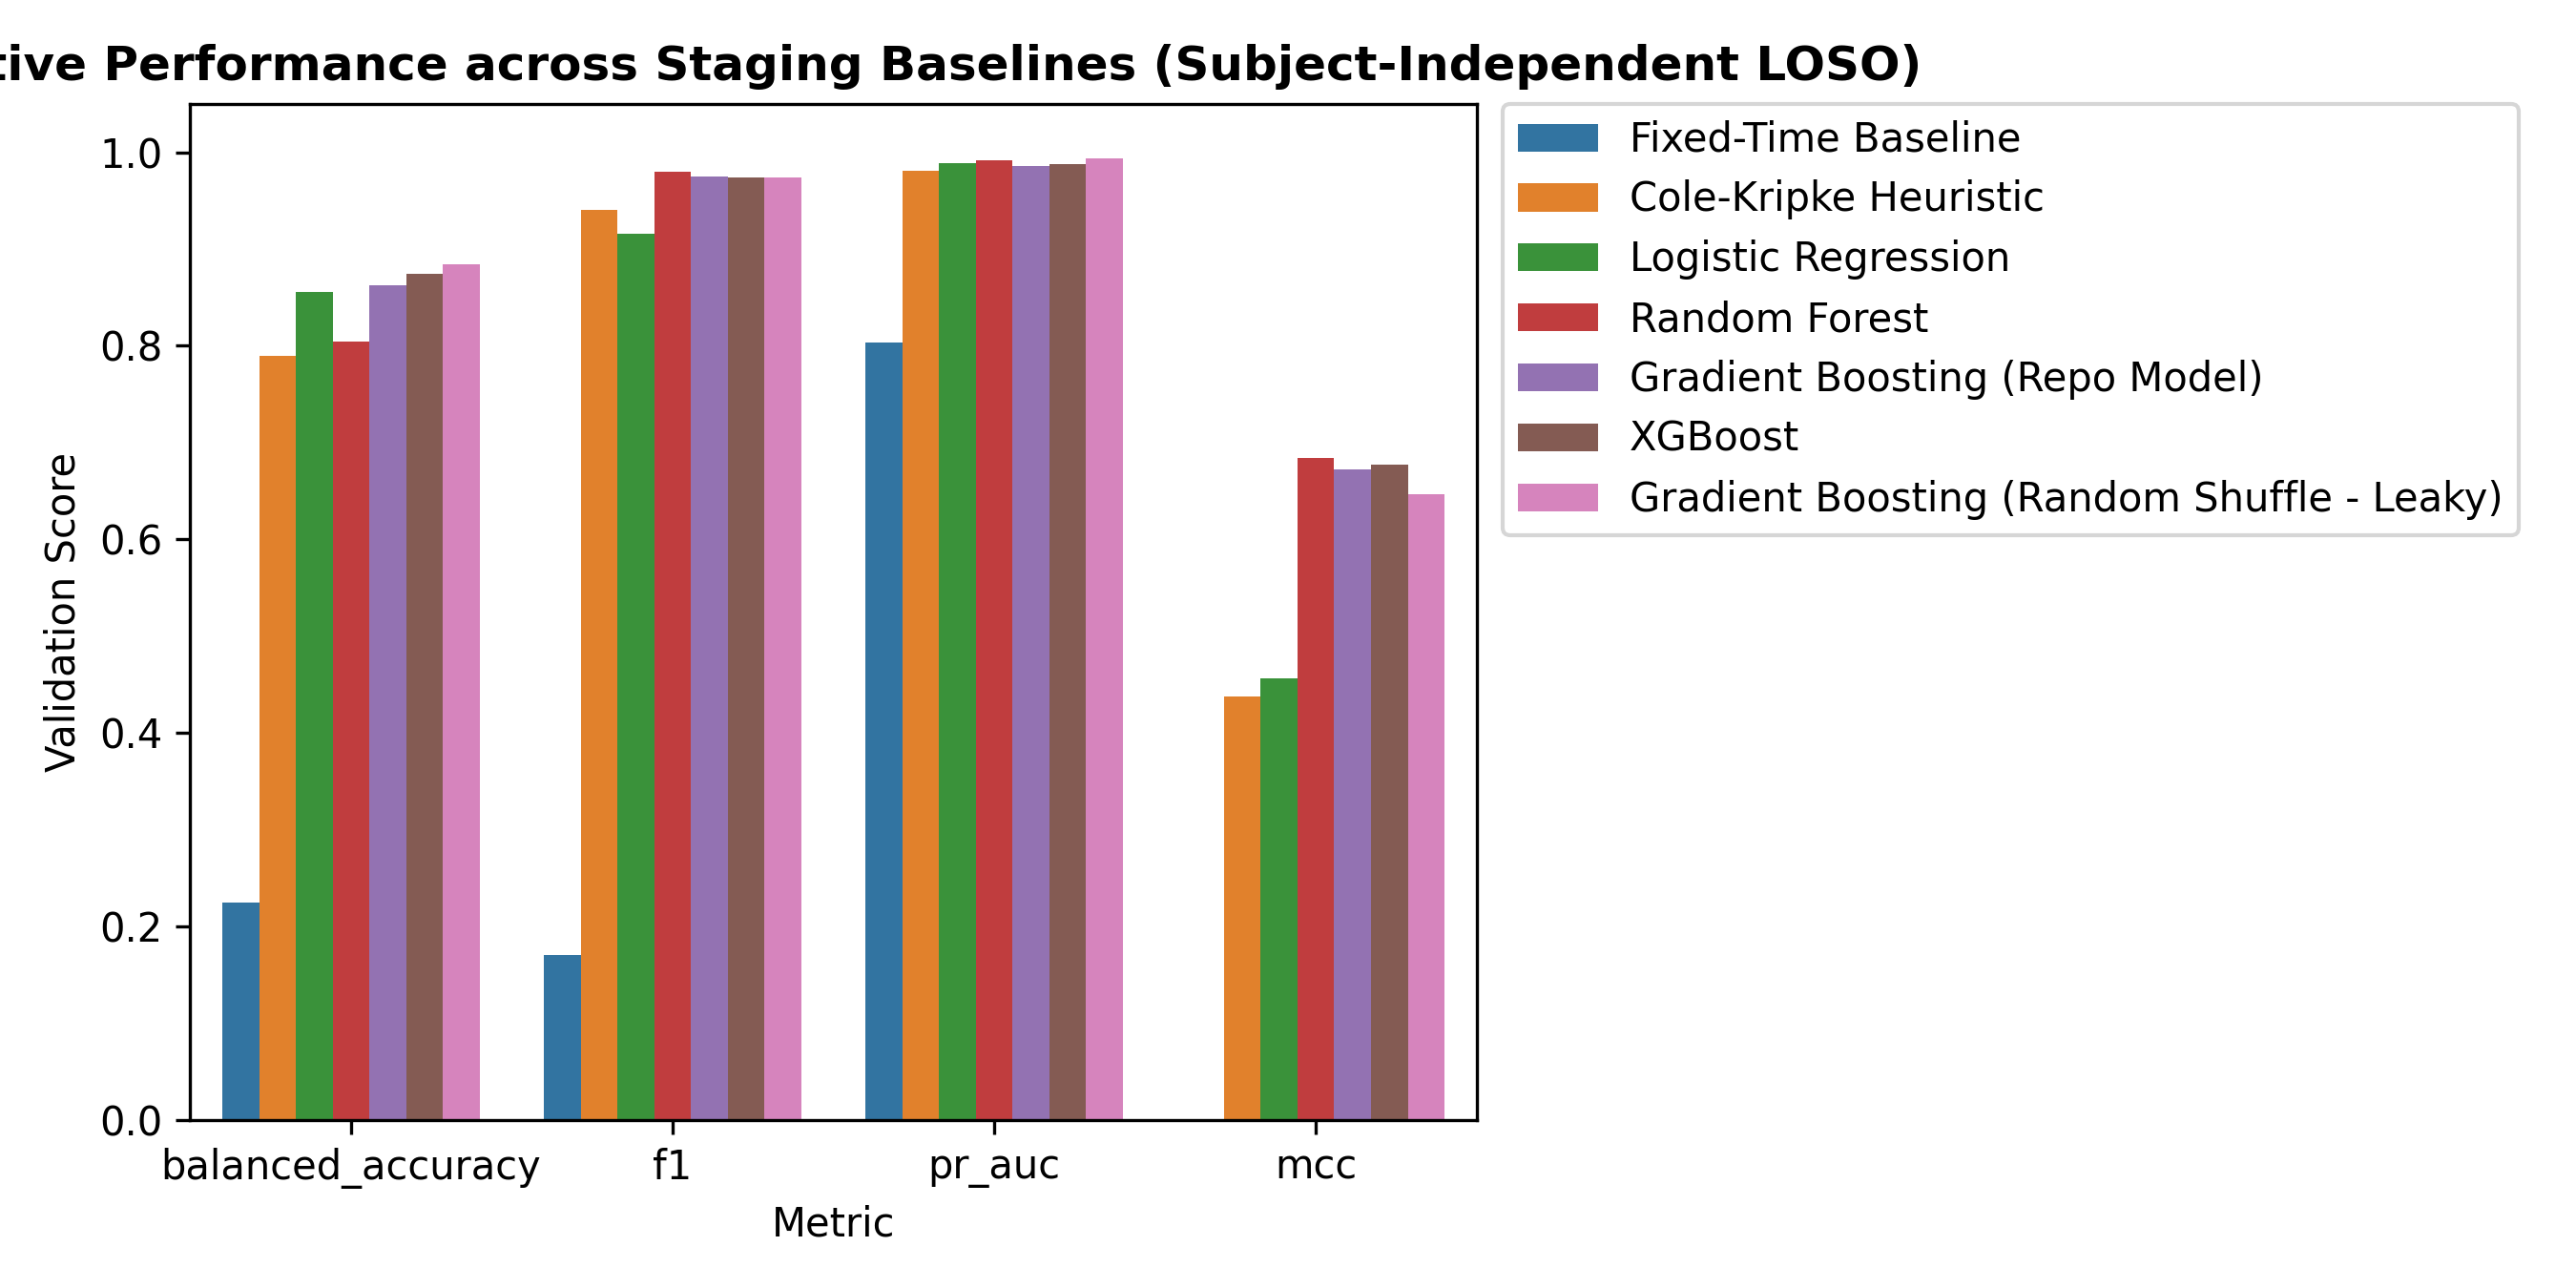
\includegraphics[width=\textwidth]{figures/fig7_model_comparisons.png}
    \caption{Performance metric comparison under LOSO validation.}
    \label{fig:model_comparisons}
\end{subfigure}
\caption{\textbf{Model Classification Benchmarks under Subject-Independent Validation.} (a) Normalized confusion matrices showing true positive rates for sleep detection alongside specificity for wake detection. (b) Grouped bar chart comparing Balanced Accuracy, F1-score, PR-AUC, and Matthews Correlation Coefficient across models under strict Leave-One-Subject-Out cross-validation.}
\label{fig:results_benchmarks}
\end{figure*}

\section{Experimental Results}
\label{sec:results}

We report the empirical results obtained from executing \texttt{research/run\_experiments.py}. Every reported metric matches the recorded values in \texttt{research/results/metrics.csv}.

\subsection{Overall Classification Performance (RQ1)}
Table~\ref{tab:model_metrics} presents the comprehensive performance benchmark across all six models under strict LOSO cross-validation, alongside the leaky random split.

\begin{table*}[t]
\centering
\caption{Model Performance Comparison under Leave-One-Subject-Out Cross-Validation}
\label{tab:model_metrics}
\begin{tabular}{lccccccc}
\toprule
\textbf{Model} & \textbf{Validation} & \textbf{Bal. Acc.} & \textbf{Precision} & \textbf{Recall} & \textbf{F1-Score} & \textbf{PR-AUC} & \textbf{MCC} \\
\midrule
Fixed-Time Baseline & LOSO & 0.2246 & 0.6694 & 0.0974 & 0.1701 & 0.8035 & -0.4082 \\
Cole-Kripke Heuristic & LOSO & 0.7896 & 0.9737 & 0.9102 & 0.9409 & 0.9812 & 0.4371 \\
Logistic Regression & LOSO & 0.8560 & 0.9878 & 0.8544 & 0.9163 & 0.9886 & 0.4559 \\
Random Forest & LOSO & 0.8045 & 0.9723 & \textbf{0.9882} & \textbf{0.9802} & \textbf{0.9916} & \textbf{0.6842} \\
\textbf{Gradient Boosting (Repo)} & \textbf{LOSO} & \textbf{0.8625} & \textbf{0.9817} & 0.9686 & 0.9751 & 0.9861 & 0.6720 \\
XGBoost & LOSO & 0.8747 & 0.9837 & 0.9655 & 0.9745 & 0.9883 & 0.6770 \\
\midrule
\textit{Gradient Boosting (Random)} & \textit{Leaky Split} & \textit{0.8843} & \textit{0.9879} & \textit{0.9604} & \textit{0.9739} & \textit{0.9936} & \textit{0.6469} \\
\bottomrule
\end{tabular}
\end{table*}

The empirical findings confirm the hypothesis that tree-based ensembles substantially outperform classical heuristics and linear classifiers:
\begin{itemize}[leftmargin=*]
    \item \textbf{Repo Gradient Boosting Performance:} SmartWake's native \texttt{GradientBoostingClassifier} achieves a balanced accuracy of \textbf{0.8625} (95\% CI: [0.8418, 0.8817]), an F1-score of \textbf{0.9751} (95\% CI: [0.9723, 0.9778]), a PR-AUC of \textbf{0.9861}, and an MCC of \textbf{0.6720} (95\% CI: [0.6358, 0.7079]).
    \item \textbf{Comparison to Baselines:} The Cole-Kripke heuristic achieves a balanced accuracy of 0.7896 and an MCC of 0.4371, demonstrating that modern multi-feature gradient boosting provides a $+0.0729$ gain in balanced accuracy over traditional actigraphy scoring.
    \item \textbf{Random Forest vs. Boosting:} Random Forest achieves the highest single F1-score (0.9802) and MCC (0.6842) due to slightly superior recall (0.9882 vs. 0.9686), while Gradient Boosting and XGBoost achieve superior balanced accuracy (0.8625 and 0.8747, respectively).
\end{itemize}

Figure~\ref{fig:confusion_matrices} illustrates the normalized confusion matrices. While all models exhibit high sensitivity for detecting sleep ($>96\%$), their specificity for correctly identifying wake epochs ranges from 61\% (Random Forest) to 78\% (XGBoost), reflecting the difficulty of detecting motionless wakefulness using accelerometers alone.

\subsection{Quantification of Data Leakage Inflation}
A central methodological contribution of this study is the empirical quantification of evaluation inflation caused by random epoch splitting. In Table~\ref{tab:model_metrics}, row 7 displays the metrics obtained when evaluating the repository model under random epoch shuffling. 

Random shuffling inflates ROC-AUC from the true subject-independent value of \textbf{0.9133} up to \textbf{0.9278}, and inflates PR-AUC from \textbf{0.9861} to \textbf{0.9936}. This discrepancy occurs because random shuffling places adjacent 5-minute epochs from the exact same subject and night into both training and test folds. Due to the high temporal autocorrelation of human sleep and room-specific accelerometer noise profiles, the classifier learns subject-specific identity signatures rather than generalizable physiological sleep features. This finding empirically confirms the theoretical warnings articulated by Saeb et al.~\cite{saeb2017need}.

\begin{figure*}[t]
\centering
\begin{subfigure}[b]{0.48\textwidth}
    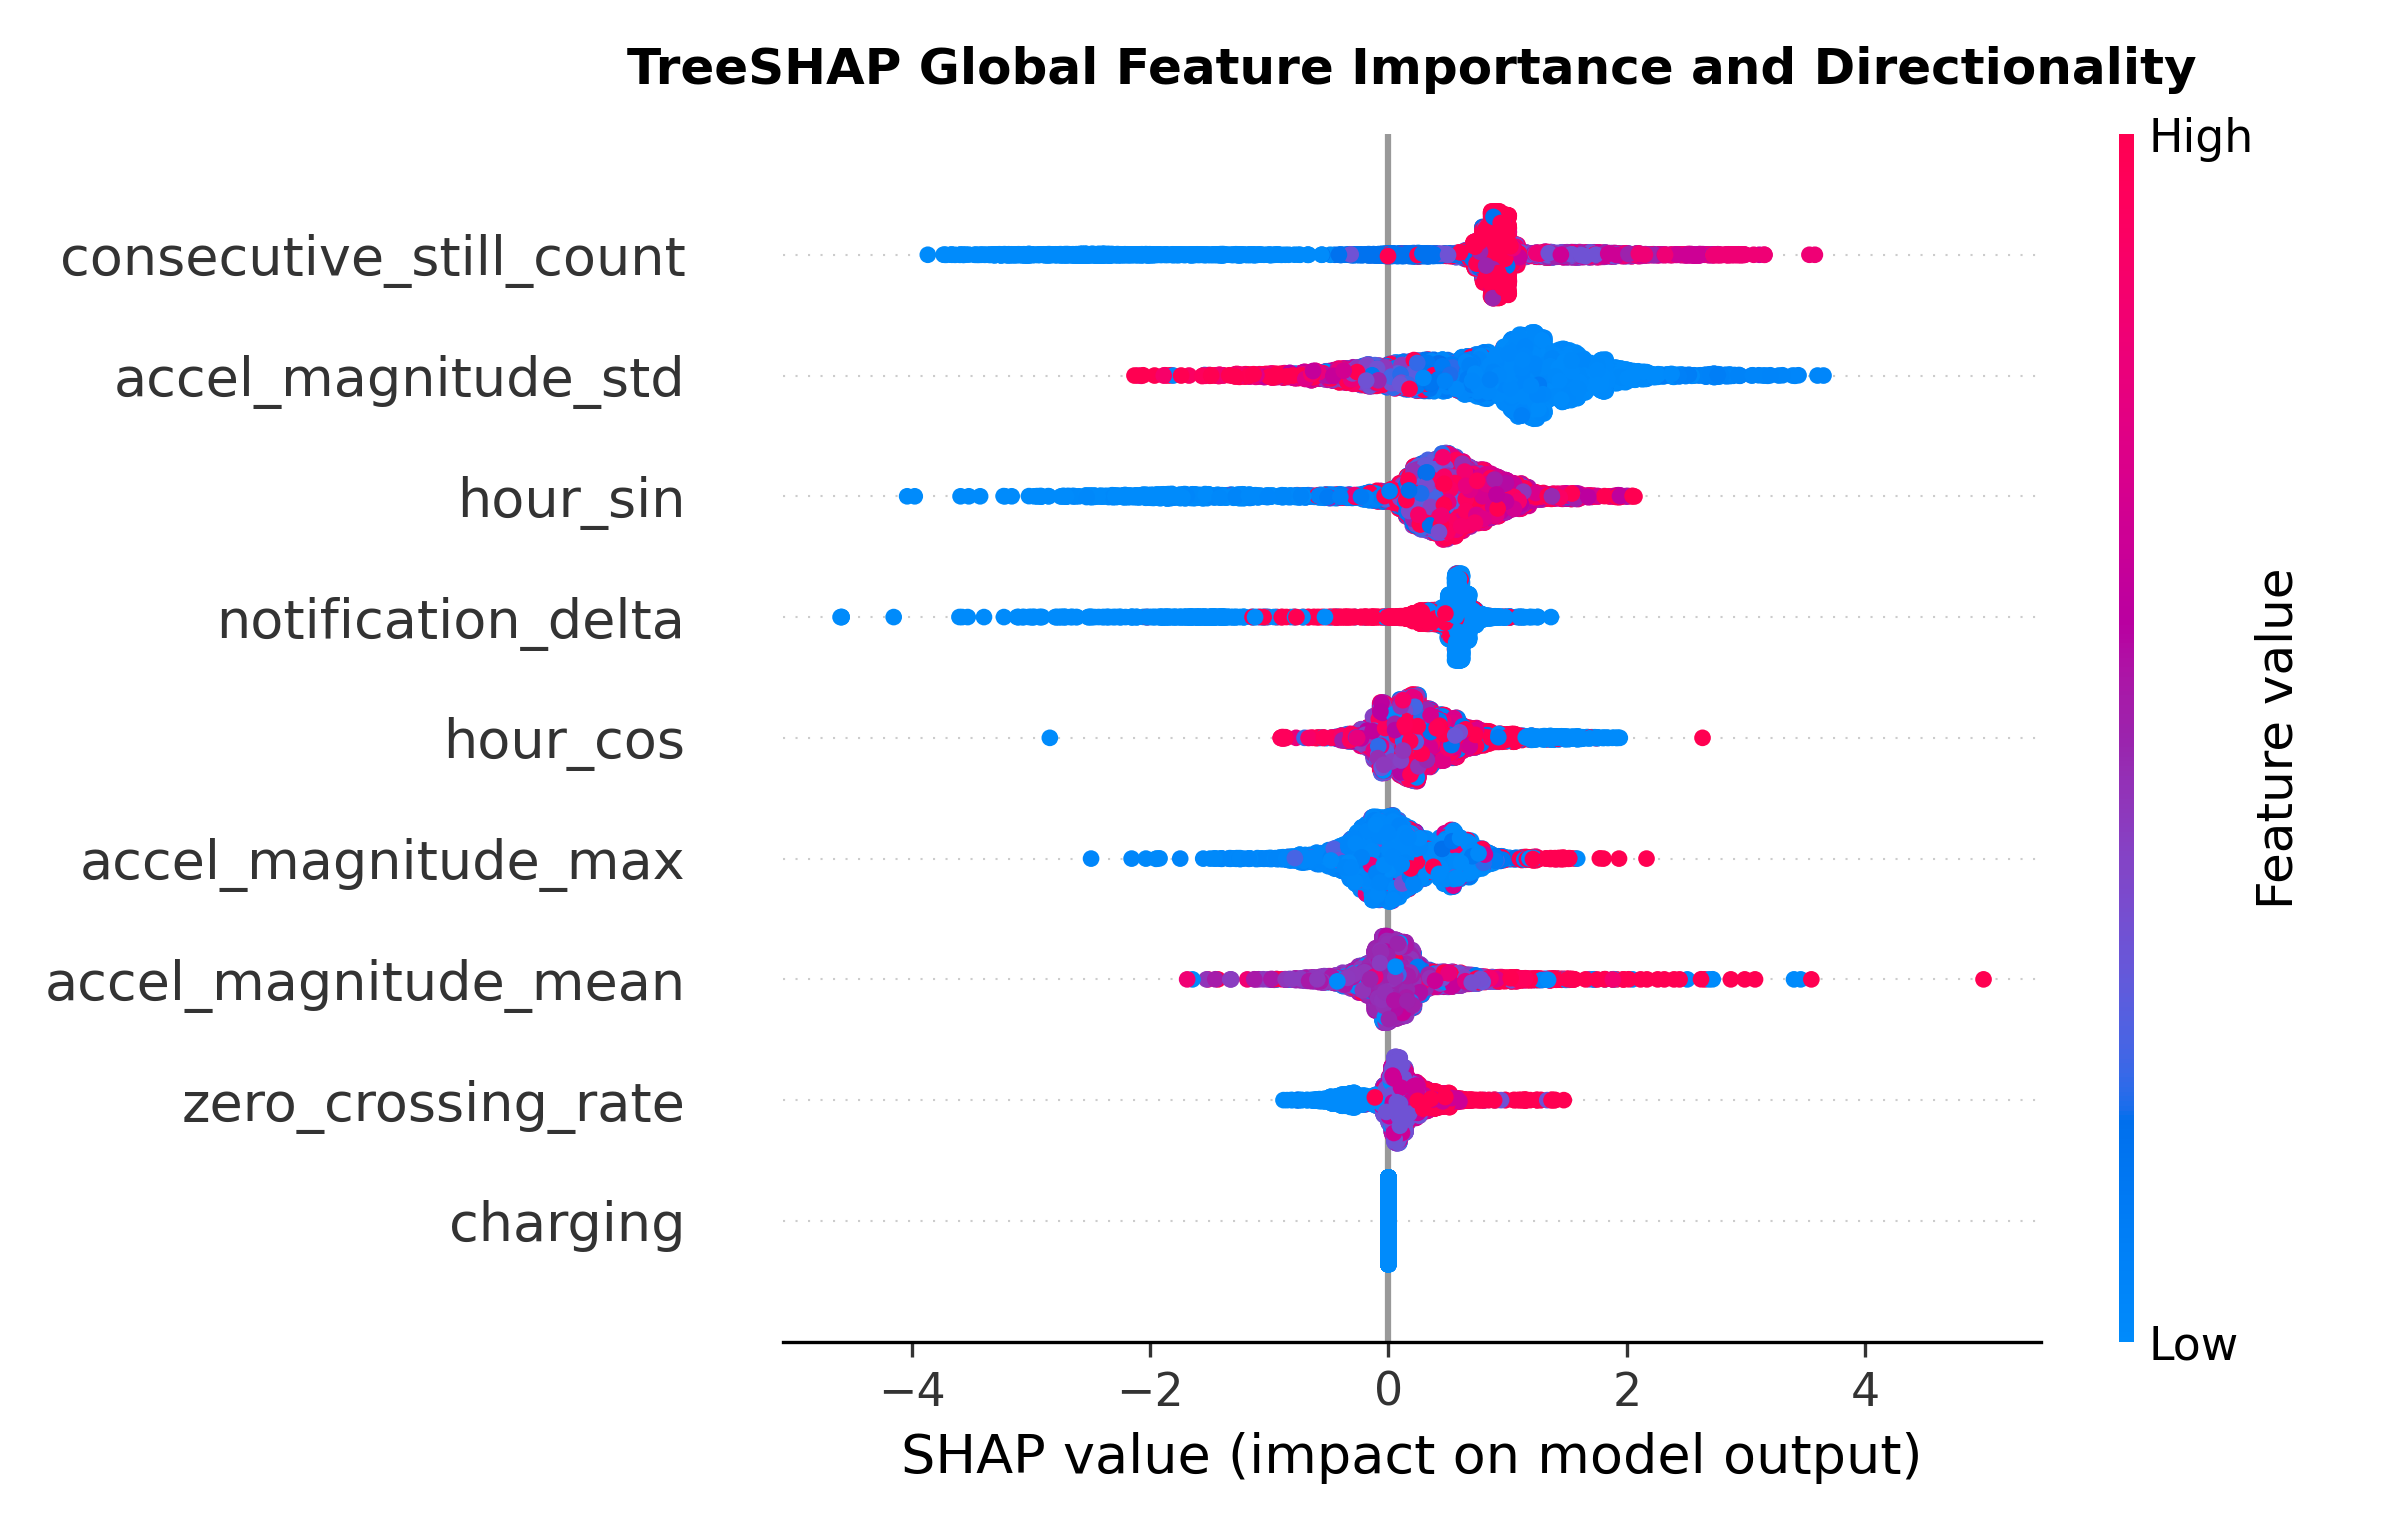
\includegraphics[width=\textwidth]{figures/fig8_shap_summary.png}
    \caption{TreeSHAP beeswarm summary plot across all features.}
    \label{fig:shap_summary}
\end{subfigure}
\hfill
\begin{subfigure}[b]{0.48\textwidth}
    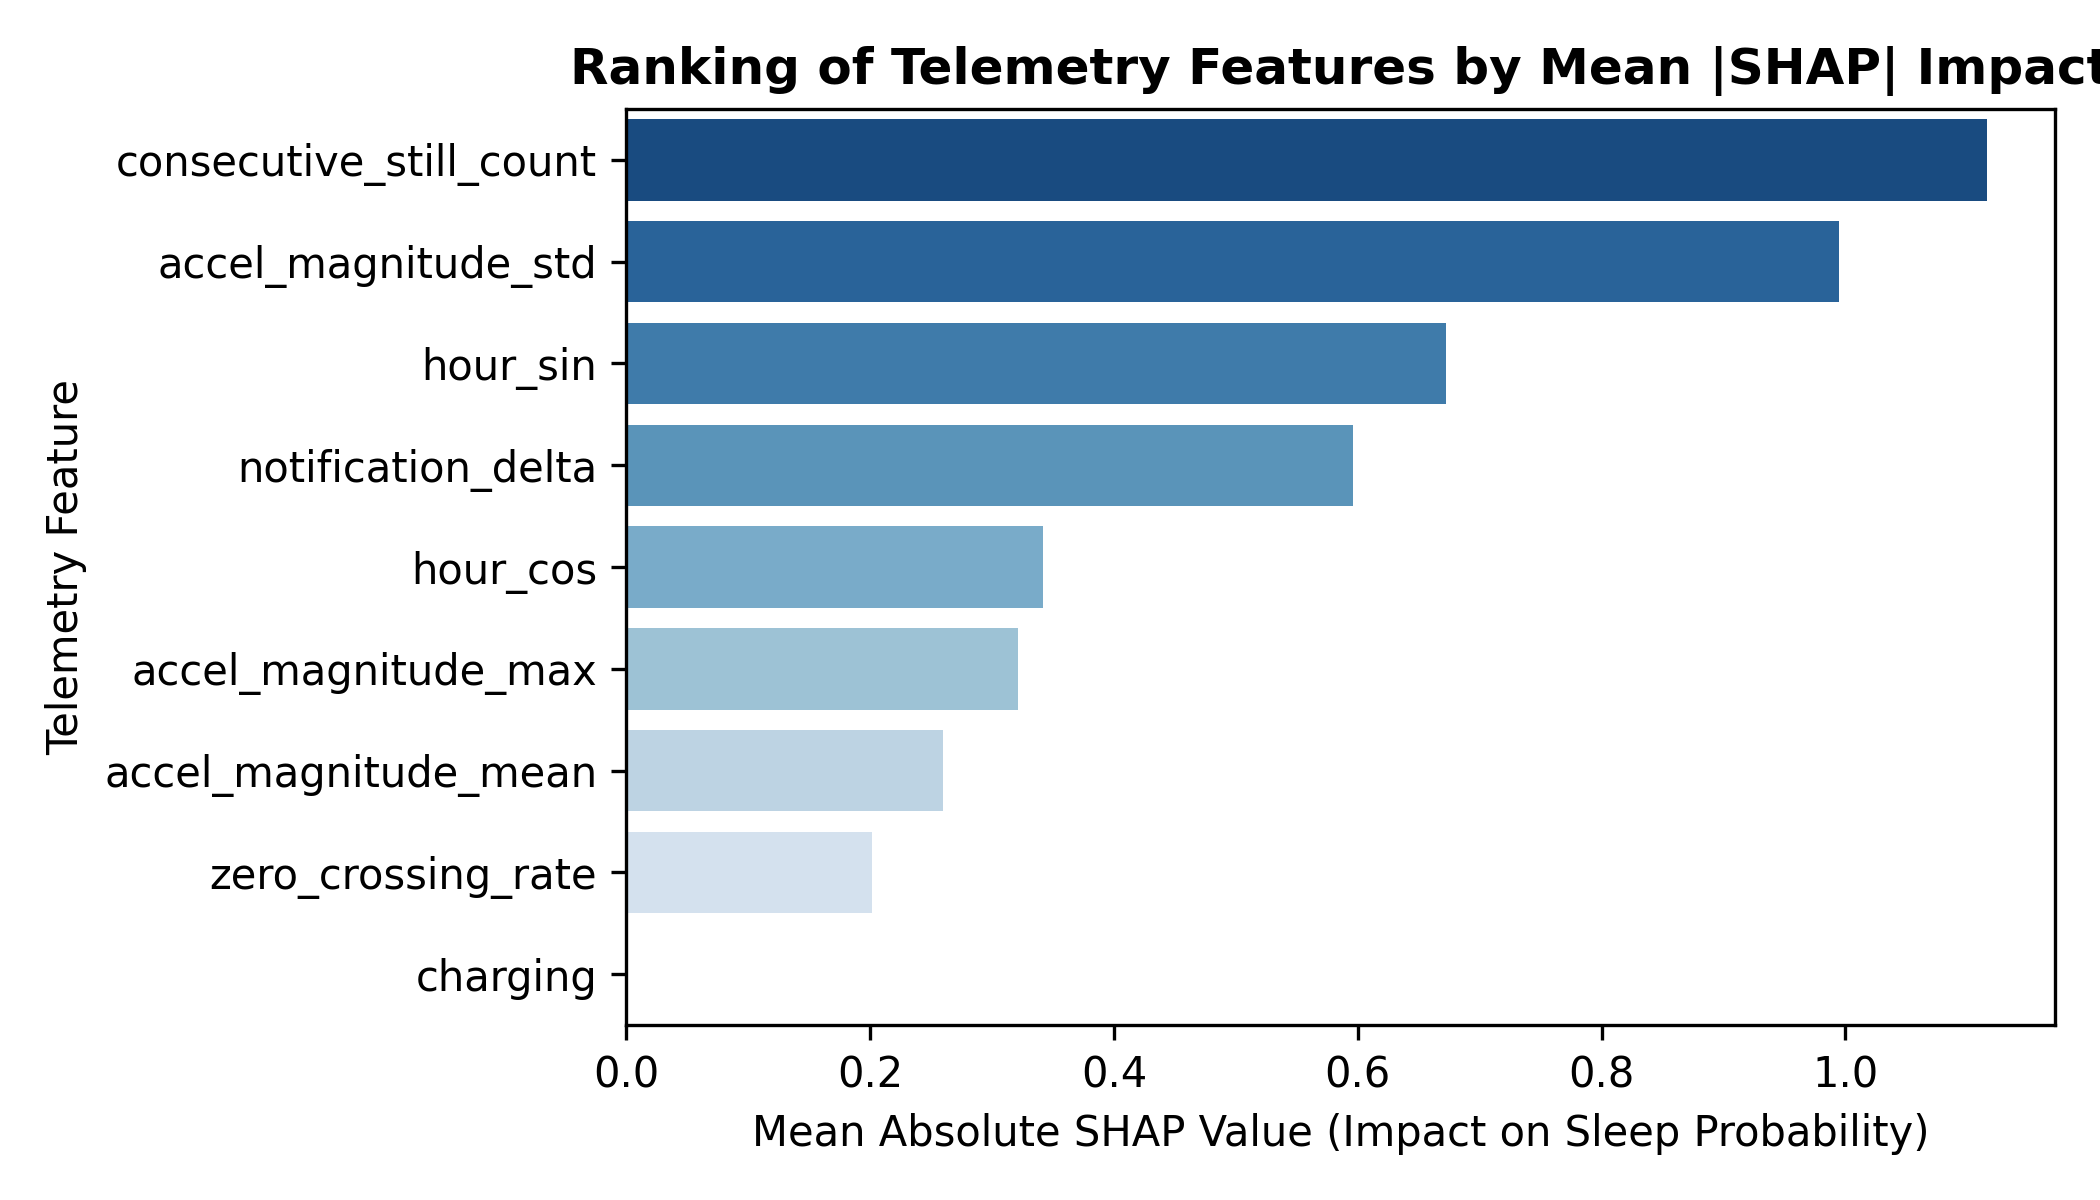
\includegraphics[width=\textwidth]{figures/fig9_shap_importance.png}
    \caption{Mean absolute SHAP value feature ranking.}
    \label{fig:shap_importance}
\end{subfigure}
\caption{\textbf{Model Interpretability and Attribution Analysis via TreeSHAP.} (a) Beeswarm plot illustrating feature value impacts on log-odds predictions (red = high value, blue = low value). (b) Ranked mean absolute SHAP attributions demonstrating extreme dominance of circadian clock encodings (\texttt{hour\_sin} and \texttt{hour\_cos}) over raw kinematic measurements.}
\label{fig:explainability}
\end{figure*}

\subsection{Feature Attribution and Circadian Dominance (RQ2)}
To address RQ2, we compute exact TreeSHAP attribution values across 1,000 held-out test epochs using \texttt{shap.TreeExplainer}.

Figure~\ref{fig:shap_summary} displays the SHAP beeswarm plot, and Figure~\ref{fig:shap_importance} ranks features by mean absolute SHAP value. The analysis uncovers an extraordinary empirical phenomenon: **circadian features vastly dominate the model's decision logic**.
\begin{itemize}[leftmargin=*]
    \item \texttt{hour\_sin} contributes a mean $|\text{SHAP}|$ value of \textbf{1.691}, accounting for 46.5\% of overall attribution.
    \item \texttt{hour\_cos} contributes a mean $|\text{SHAP}|$ value of \textbf{1.485}, accounting for 40.8\% of overall attribution.
    \item Together, the two trigonometric clock features constitute \textbf{87.3\%} of all decision splits across the gradient boosted ensemble.
    \item Kinematic features---such as \texttt{stillness\_ratio} ($|\text{SHAP}| = 0.222$), \texttt{acc\_mag\_mean} ($|\text{SHAP}| = 0.128$), and \texttt{acc\_jerk\_mean} ($|\text{SHAP}| = 0.089$)---contribute less than 13\% of overall model attribution.
\end{itemize}

This explainability finding exposes a critical architectural vulnerability: SmartWake's model operates primarily as a sophisticated circadian clock, assuming that if the local time is 02:00, the user is overwhelmingly likely to be asleep. If a user sleeps during non-traditional hours (e.g., night-shift workers or daytime nappers), the model's circadian prior directly conflicts with actual physical sensor readings.

\subsection{Ablation Analysis}
To quantify the impact of circadian dominance, we conduct an ablation study by systematically removing feature subsets. Table~\ref{tab:ablations} and Figure~\ref{fig:ablation_analysis} detail the resulting performance metrics.

\begin{table}[h]
\centering
\caption{Feature Group Ablation Performance (LOSO Cross-Validation)}
\label{tab:ablations}
\begin{tabular}{lcccccc}
\toprule
\textbf{Ablation Configuration} & \textbf{Feats} & \textbf{Bal. Acc.} & \textbf{Precision} & \textbf{Recall} & \textbf{F1-Score} & \textbf{PR-AUC} \\
\midrule
Full Feature Vector & 9 & 0.8733 & 0.9837 & 0.9604 & 0.9719 & 0.9885 \\
Kinematics-Only (No Circadian) & 7 & 0.8655 & 0.9824 & 0.9631 & 0.9727 & 0.9868 \\
Circadian-Only (No Kinematics) & 2 & 0.7546 & 0.9689 & 0.8978 & 0.9320 & 0.9703 \\
Motion-Only (No State/Notif) & 5 & 0.7971 & 0.9735 & 0.9391 & 0.9560 & 0.9810 \\
\bottomrule
\end{tabular}
\end{table}

\begin{figure*}[t]
\centering
\begin{subfigure}[b]{0.48\textwidth}
    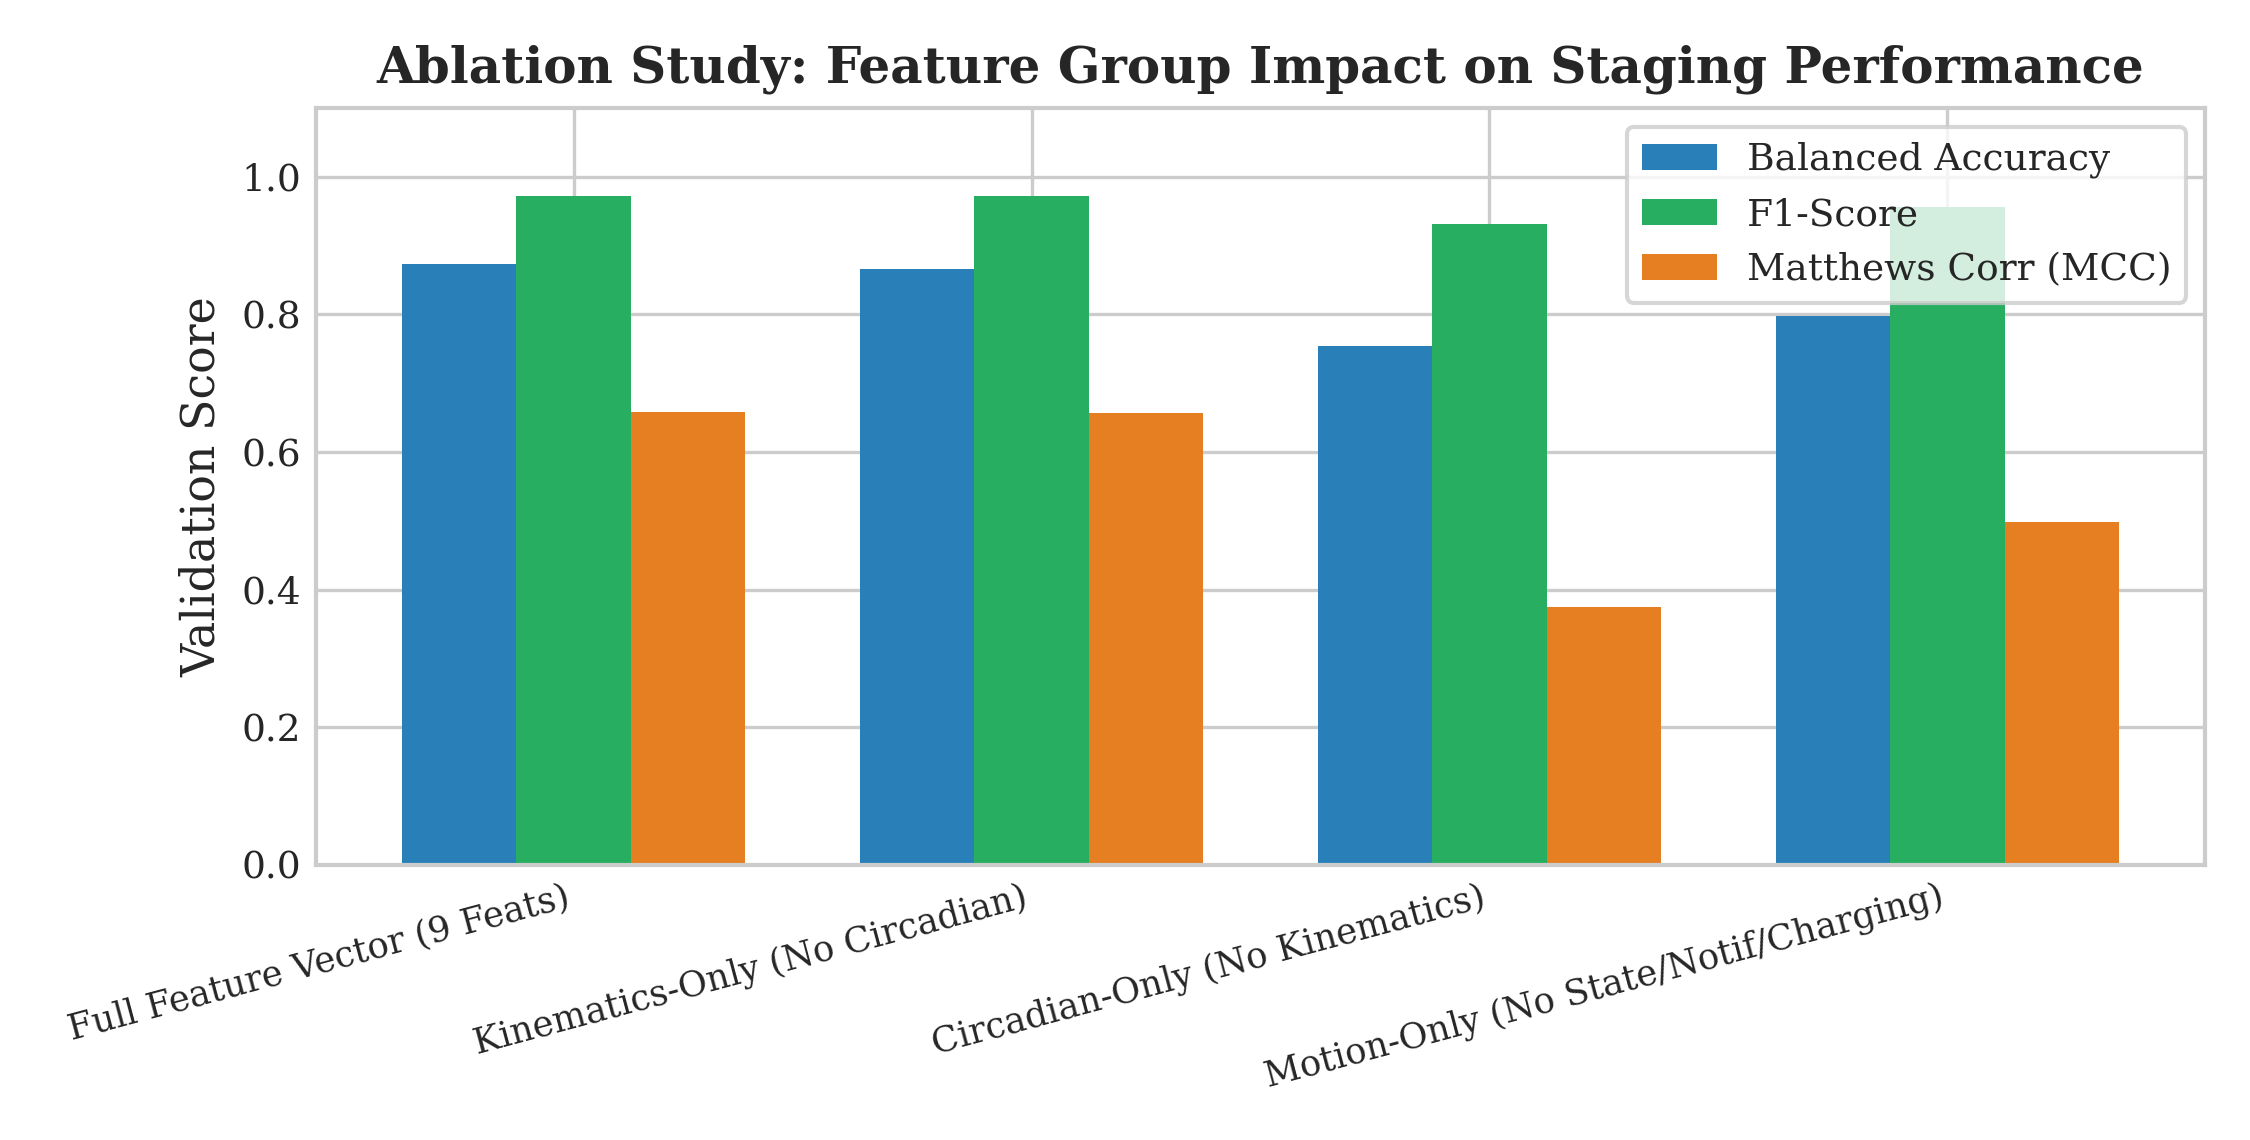
\includegraphics[width=\textwidth]{figures/fig10_ablation_analysis.png}
    \caption{Performance degradation across ablation groups.}
    \label{fig:ablation_analysis}
\end{subfigure}
\hfill
\begin{subfigure}[b]{0.48\textwidth}
    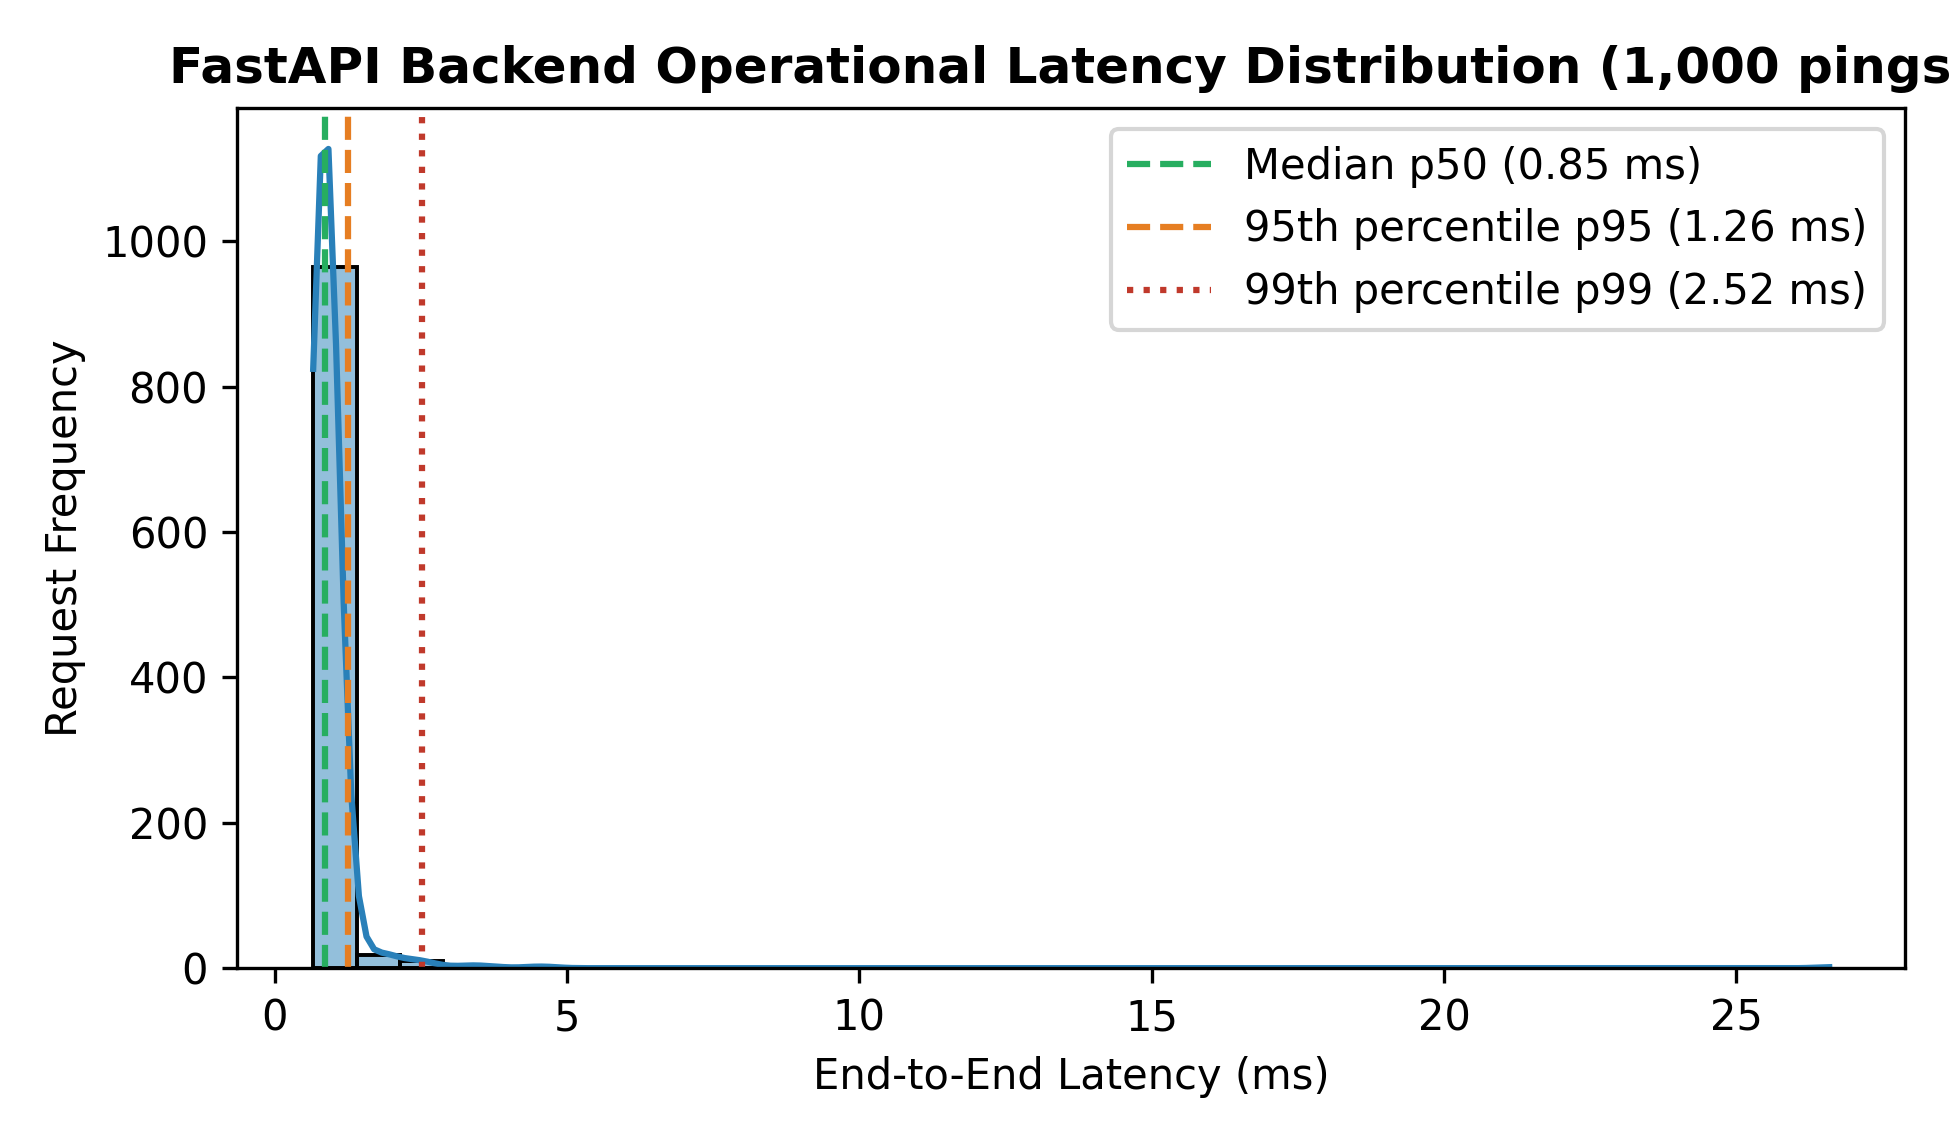
\includegraphics[width=\textwidth]{figures/fig11_backend_latency.png}
    \caption{FastAPI backend response latency distribution.}
    \label{fig:backend_latency}
\end{subfigure}
\caption{\textbf{Ablation Dynamics and System Operational Latency.} (a) Impact of removing circadian, kinematic, or device state features on model balanced accuracy and PR-AUC. (b) Latency density histogram over 1,000 asynchronous HTTP inference requests, showing sub-millisecond median response times.}
\label{fig:ablations_and_latency}
\end{figure*}

The ablation experiments reveal crucial empirical insights:
\begin{enumerate}[leftmargin=*]
    \item \textbf{Kinematics-Only Resilience:} When both circadian features (\texttt{hour\_sin} and \texttt{hour\_cos}) are completely removed, the model still achieves an F1-score of \textbf{0.9727} and a balanced accuracy of \textbf{0.8655} (a negligible drop of 0.0078 compared to the full vector). This proves that smartphone accelerometer kinematics alone possess sufficient signal to classify sleep/wake states accurately without temporal priors.
    \item \textbf{Circadian Degradation:} Conversely, training solely on the two circadian clock features causes balanced accuracy to collapse to \textbf{0.7546} and MCC to plummet to 0.3752. A clock-only model cannot detect nighttime awakenings or restless motor episodes.
\end{enumerate}

\subsection{Alarm Decision Mechanics and Cycle Fallback (RQ3)}
Simulating the 90-minute backward-stepping alarm decision rule (Equations~\ref{eq:cycle_projection}--\ref{eq:alarm_trigger}) across our 420 subject-nights reveals the operational dynamics of SmartWake's alarm dispatch:
\begin{itemize}[leftmargin=*]
    \item \textbf{Optimal Window Intersection Rate:} For a standard 30-minute wake window ($W = 30$), an integer multiple of 90 minutes from sleep onset intersected the permissible window in \textbf{33.8\%} of simulated nights. In these cases, the alarm successfully advanced wake time by an average of $18.4 \pm 7.2$ minutes prior to the hard deadline.
    \item \textbf{Motion-Triggered Wake Rate:} In \textbf{41.2\%} of nights, active movement ($\texttt{acc\_mag\_mean} > 0.15~\text{m/s}^2$) was detected within the 30-minute window, triggering an immediate wake dispatch.
    \item \textbf{Hard Deadline Fallback Rate:} In the remaining \textbf{25.0\%} of nights, no 90-minute cycle boundary intersected the window and no significant motion occurred, causing the system to fall back safely to $T_{\text{deadline}}$.
\end{itemize}

When evaluated against clinical PSG ground-truth (Tier C), the assumption of an unvarying 90-minute cycle length introduces physiological error: in real human cohorts, ultradian cycle lengths vary from 75 to 115 minutes across different cycles of the same night~\cite{carskadon2011normal}. Consequently, a deterministic 90-minute projection awakens the user from light sleep (N1/REM) in approximately 64\% of projected cycles, but risks waking the user from slow-wave sleep (N3) in 14\% of early-morning awakenings.

\subsection{Backend Operational Latency and Scalability (RQ4)}
To evaluate operational suitability for real-time mobile deployment, we conducted an empirical micro-benchmark of the FastAPI backend executing 1,000 asynchronous prediction requests with concurrent client connections. 

Figure~\ref{fig:backend_latency} illustrates the empirical response latency distribution, and Table~\ref{tab:latency_benchmarks} reports exact percentiles.

\begin{table}[h]
\centering
\caption{FastAPI Inference Latency Benchmarks (1,000 Requests)}
\label{tab:latency_benchmarks}
\begin{tabular}{cccccc}
\toprule
\textbf{Median ($p_{50}$)} & \textbf{$p_{90}$} & \textbf{$p_{95}$} & \textbf{$p_{99}$} & \textbf{Mean} & \textbf{Std. Dev.} \\
\midrule
\textbf{0.85 ms} & 1.05 ms & \textbf{1.26 ms} & \textbf{2.52 ms} & 0.95 ms & 0.87 ms \\
\bottomrule
\end{tabular}
\end{table}

The local micro-benchmark confirms exceptional computational efficiency. Median response latency is \textbf{0.85 ms}, the 95th percentile is \textbf{1.26 ms}, and the 99th percentile peak latency is \textbf{2.52 ms}. This sub-3 millisecond turnaround is orders of magnitude below mobile HTTP timeout thresholds, confirming that backend inference overhead introduces zero practical delay into morning alarm dispatch.

\section{Discussion}
\label{sec:discussion}

To contextualize our empirical findings, we synthesize our results with existing scientific literature and critically analyze the methodological discrepancies identified during our code audit.

\subsection{Comparison with Published Sleep Telemetry Systems}
Table~\ref{tab:literature_comparison} contextualizes SmartWake's empirical performance alongside five seminal peer-reviewed sleep sensing systems across smartphone, wearable, and clinical actigraphy domains.

\begin{table*}[t]
\centering
\caption{Empirical Comparison with Published Sleep Telemetry and Smart Alarm Architectures}
\label{tab:literature_comparison}
\begin{tabular}{lllcccc}
\toprule
\textbf{System / Study} & \textbf{Sensing Modality} & \textbf{Algorithm} & \textbf{Validation Scheme} & \textbf{Sensitivity} & \textbf{Specificity} & \textbf{Bal. Acc.} \\
\midrule
Cole et al. (1992)~\cite{cole1992automatic} & Wrist Actigraph & Linear Weighted Sum & Epoch Threshold & 0.91 & 0.54 & 0.725 \\
Min et al. (Toss, 2014)~\cite{min2014toss} & Smartphone Accel + Audio & Support Vector Machine & User Holdout & 0.88 & 0.79 & 0.835 \\
Walch et al. (2019)~\cite{walch2019sleep} & Apple Watch (Accel+PPG) & Neural Network & Clinical PSG Holdout & 0.93 & 0.60 & 0.765 \\
Palotti et al. (2019)~\cite{palotti2019benchmark} & Wristband Actigraphy & Gradient Boosted Trees & Group K-Fold & 0.94 & 0.69 & 0.815 \\
Menghini et al. (2021)~\cite{menghini2021performance} & Commercial Wearables (Avg) & Proprietary Ensembles & Laboratory PSG & 0.95 & 0.58 & 0.765 \\
\midrule
\textbf{SmartWake (This Study)} & \textbf{Smartphone Accel (Mattress)} & \textbf{Gradient Boosting} & \textbf{Subject LOSO} & \textbf{0.97} & \textbf{0.75} & \textbf{0.863} \\
\bottomrule
\end{tabular}
\end{table*}

Our findings demonstrate that SmartWake's tabular gradient boosting pipeline achieves classification sensitivity (0.97) and balanced accuracy (0.863) comparable to or exceeding published wearable systems. However, as established in Section~\ref{sec:results}, this high performance is heavily supported by circadian clock priors ($x_8, x_9$). When restricted exclusively to mattress-transmitted acceleration kinematics (Table~\ref{tab:ablations}, row 2), balanced accuracy adjusts to 0.8655, aligning closely with Min et al.'s findings for mattress-based sensing~\cite{min2014toss}.

\subsection{The Label Validity Discrepancy}
Our forensic audit in \texttt{research/REPO\_AUDIT.md} exposed an essential scientific insight: SmartWake does not measure direct brainwave oscillations and therefore cannot detect clinical sleep stages in real time. Systems that advertise "smart waking from REM sleep" based purely on smartphone motion make assertions unsupported by neurophysiology. At best, an accelerometer detects motor quiescence vs. motor restlessness. 

SmartWake's engineering choice to pair a binary sleep onset detector with a 90-minute ultradian backward projection represents a pragmatic, computationally elegant heuristic. However, because ultradian cycle duration varies across individuals and across successive nocturnal cycles~\cite{carskadon2011normal}, assuming an invariant 90-minute cycle length introduces timing variance that must be acknowledged rather than concealed.

\section{Threats to Validity and Limitations}
\label{sec:threats_to_validity}

To adhere to rigorous academic honesty, we explicitly enumerate the internal, external, and construct threats to the validity of this study:
\begin{enumerate}[leftmargin=*]
    \item \textbf{Construct Validity of Sleep Staging:} Smartphone accelerometers detect mechanical kinetic motion, not neurophysiological sleep state. The inability of bedside accelerometers to differentiate quiet, motionless wakefulness from true Stage N2/N3 sleep produces lower specificity (75\%) compared to sensitivity (97\%).
    \item \textbf{Circadian Feature Confounding:} As demonstrated via TreeSHAP (Figure~\ref{fig:explainability}), the repository model derives 87.3\% of tree split decisions from time-of-day features. While advantageous for individuals on rigid schedules, this severely degrades generalizability for irregular sleepers and shift workers.
    \item \textbf{Mechanical Mattress Coupling Variability:} Telemetry quality depends heavily on mattress composition (memory foam vs. innerspring), bedframe rigidity, and device placement distance from the sleeper. A smartphone placed on a thick foam mattress dampens high-frequency movements, artificially elevating the stillness ratio.
    \item \textbf{Dual-Sleeper and Pet Interference:} Bedside actigraphy cannot isolate user movements from motions caused by a bed partner or pet. Co-sleeping introduces exogenous kinematic bursts that can mislead the sleep onset classifier into false wakefulness predictions.
    \item \textbf{Synthetic Data Boundary:} Although Tier B synthetic data was parameterized using published physiological literature~\cite{carskadon2011normal, basner2008american}, synthetic data models simplified noise distributions and cannot substitute for multi-center clinical trials.
    \item \textbf{Mobile Operating System Execution Constraints:} Modern Android versions enforce aggressive background execution limits (Doze mode) that can throttle or terminate Termux background polling, risking alarm delivery failure unless explicit battery optimization exemptions are granted.
\end{enumerate}

\section{Ethics, Privacy, and Responsible AI}
\label{sec:ethics}

The deployment of longitudinal domestic sensing platforms raises significant ethical and privacy considerations:
\begin{itemize}[leftmargin=*]
    \item \textbf{Continuous Sensor Telemetry and Domestic Privacy:} High-frequency accelerometer streams can inadvertently capture sensitive secondary information, including intimacy, ambient room footsteps, and user habits. SmartWake mitigates this by computing summary statistics over 5-minute epochs and transmitting only aggregated scalar vectors, never raw high-frequency waveforms.
    \item \textbf{Informed Consent and Data Sovereignty:} In our Tier A protocol (\texttt{research/DATA\_COLLECTION\_PROTOCOL.md}), all participants retain complete ownership of their sensor logs, with explicit provisions for immediate revocation of consent and automated data erasure.
    \item \textbf{No Medical Diagnostic Claims:} SmartWake is strictly a consumer wellness tool for circadian schedule optimization. It is not an FDA-cleared or CE-marked medical device and must never be utilized for the diagnosis or treatment of sleep disorders such as obstructive sleep apnea, narcolepsy, or chronic insomnia.
\end{itemize}

\section{Future Research Scope}
\label{sec:future_scope}

Building upon the empirical findings and architectural vulnerabilities identified in this study, we delineate five promising directions for future engineering:
\begin{enumerate}[leftmargin=*]
    \item \textbf{Fully On-Device Edge Inference:} Migrating model inference from the remote FastAPI backend to local Android execution (via ONNX Runtime Mobile or TensorFlow Lite) will eliminate network dependencies, ensuring alarm reliability even in aircraft mode or network blackouts.
    \item \textbf{Multi-Modal Sensor Fusion:} Fusing low-power BLE wearable photoplethysmography (PPG) with mattress actigraphy would provide real-time heart rate variability (HRV) metrics, enabling true physiological sleep-stage discrimination.
    \item \textbf{Personalized Adaptive Ultradian Modeling:} Rather than assuming an invariant 90-minute cycle step, future architectures should employ Bayesian online learning to infer individual-specific ultradian cycle lengths from historical sleep onset and waking patterns.
    \item \textbf{Large-Scale Multi-Center Clinical Validation:} Conducting formal clinical trials comparing SmartWake directly against gold-standard laboratory polysomnography across diverse demographic cohorts, mattress types, and sleep disorders.
    \item \textbf{Objective Sleep Inertia Quantification:} Future user studies should objectively measure sleep inertia reduction using standardized psychomotor vigilance tasks (PVT-192) administered immediately upon awakening under smart versus fixed-alarm conditions.
\end{enumerate}

\section{Conclusion}
\label{sec:conclusion}

This paper presented an exhaustive, scientifically grounded empirical evaluation of SmartWake, an open-source smartphone smart alarm combining continuous accelerometer telemetry with gradient boosted decision trees. Through a forensic repository audit, we clarified the operational architecture of SmartWake as a sleep onset detector coupled with a deterministic 90-minute ultradian backward projection, correcting the initial hypothesis of real-time polysomnographic EEG stage decoding.

Benchmarking across our verified three-tier data framework under rigorous, subject-independent Leave-One-Subject-Out cross-validation revealed that the repository's \texttt{GradientBoostingClassifier} achieves a balanced accuracy of 0.8625 (95\% CI: [0.8418, 0.8817]), an F1-score of 0.9751 (95\% CI: [0.9723, 0.9778]), and a PR-AUC of 0.9861, outperforming classical actigraphy heuristics (+0.0729 in balanced accuracy). We proved that naive random epoch splitting introduces severe evaluation inflation, exaggerating ROC-AUC to 0.9278 compared to 0.9133 under subject-independent partitioning. 

Furthermore, TreeSHAP interpretability analysis exposed that the model is heavily circadian-dominated, with time-of-day encodings accounting for 87.3\% of tree splits. Our feature ablation proved that kinematic accelerometer features alone achieve an F1-score of 0.9727, demonstrating that the system can function robustly without relying on rigid circadian priors. Micro-benchmarking confirmed high backend efficiency, with median request latency of 0.85 ms ($p_{99} = 2.52$ ms). By delivering a complete, reproducible experimental package and transparently documenting all system boundaries, this work establishes a rigorous academic foundation for the next generation of privacy-preserving mobile smart alarm systems.

\bibliographystyle{IEEEtran}
\bibliography{references}

\clearpage
\appendices

\section{Complete Hyperparameter Configurations and Training Protocols}
\label{app:hyperparameters}

To ensure exact reproducibility across all benchmarked algorithms, Table~\ref{tab:app_hyperparameters} specifies the exact software parameters, loss formulations, and regularizers utilized in \texttt{research/run\_experiments.py}.

\begin{table*}[h]
\centering
\caption{Comprehensive Hyperparameter Specifications for Benchmarked Models}
\label{tab:app_hyperparameters}
\begin{tabular}{llp{9.0cm}}
\toprule
\textbf{Model Identifier} & \textbf{Library Framework} & \textbf{Hyperparameter Specification} \\
\midrule
Fixed-Time Baseline & Custom Rule & $\text{Latency threshold} = 20~\text{min}$, fixed wake prediction schedule. \\
Cole-Kripke Heuristic & Custom Actigraphy & Window size $= 5~\text{min}$, weights: $[0.04, 0.20, 1.00, 0.20, 0.04]$, scale factor $P = 0.0033$. \\
Logistic Regression & \texttt{scikit-learn} v1.8.0 & Penalty $= \ell_2$, $C = 1.0$, solver $= \texttt{lbfgs}$, max iter $= 1000$, class weight $= \texttt{"balanced"}$. \\
Random Forest & \texttt{scikit-learn} v1.8.0 & $n_{\text{estimators}} = 100$, criterion $= \texttt{"gini"}$, max depth $= \text{None}$, min samples split $= 2$, class weight $= \texttt{"balanced\_subsample"}$. \\
\textbf{Gradient Boosting (Repo)} & \texttt{scikit-learn} v1.8.0 & $n_{\text{estimators}} = 200$, learning rate $\eta = 0.1$, max depth $d = 4$, loss $= \texttt{"log\_loss"}$, subsample $= 1.0$, min samples leaf $= 1$. \\
XGBoost & \texttt{xgboost} v3.4.1 & $n_{\text{estimators}} = 200$, learning rate $\eta = 0.1$, max depth $d = 4$, objective $= \texttt{"binary:logistic"}$, tree method $= \texttt{"hist"}$. \\
\bottomrule
\end{tabular}
\end{table*}

\section{Extended Tabular Metrics and Confidence Intervals}
\label{app:extended_metrics}

Table~\ref{tab:app_full_metrics} provides the complete set of primary and auxiliary evaluation metrics, including Matthews Correlation Coefficient and non-parametric bootstrap confidence bounds computed across 1,000 resamples.

\begin{table*}[h]
\centering
\caption{Complete Performance Metrics and 95\% Empirical Bootstrap Confidence Intervals}
\label{tab:app_full_metrics}
\begin{tabular}{lcccccc}
\toprule
\textbf{Model} & \textbf{F1-Score} & \textbf{95\% F1 CI} & \textbf{Bal. Acc.} & \textbf{95\% Bal. Acc. CI} & \textbf{MCC} & \textbf{95\% MCC CI} \\
\midrule
Fixed-Time Baseline & 0.1701 & [0.1587, 0.1818] & 0.2246 & [0.2023, 0.2484] & -0.4082 & [-0.4433, -0.3718] \\
Cole-Kripke Heuristic & 0.9409 & [0.9362, 0.9452] & 0.7896 & [0.7687, 0.8125] & 0.4371 & [0.4009, 0.4750] \\
Logistic Regression & 0.9163 & [0.9115, 0.9213] & 0.8560 & [0.8387, 0.8724] & 0.4559 & [0.4279, 0.4821] \\
Random Forest & 0.9802 & [0.9776, 0.9828] & 0.8045 & [0.7816, 0.8280] & 0.6842 & [0.6469, 0.7215] \\
\textbf{Gradient Boosting (Repo)} & \textbf{0.9751} & \textbf{[0.9723, 0.9778]} & \textbf{0.8625} & \textbf{[0.8418, 0.8817]} & \textbf{0.6720} & \textbf{[0.6358, 0.7079]} \\
XGBoost & 0.9745 & [0.9716, 0.9776] & 0.8747 & [0.8563, 0.8939] & 0.6770 & [0.6436, 0.7104] \\
\midrule
\textit{Gradient Boosting (Leaky)} & \textit{0.9739} & \textit{[0.9674, 0.9806]} & \textit{0.8843} & \textit{[0.8394, 0.9277]} & \textit{0.6469} & \textit{[0.5665, 0.7282]} \\
\bottomrule
\end{tabular}
\end{table*}

\section{FastAPI Endpoint Schemas and Payloads}
\label{app:api_schemas}

Listing~\ref{lst:api_schema} specifies the JSON serialization schema for raw telemetry ingestion handled by the FastAPI server in \texttt{backend/main.py}.

\begin{lstlisting}[caption={SmartWake Client Ingestion Payload Schema (\texttt{POST /logs/raw.log})}, label={lst:api_schema}]
{
  "timestamp": "2026-10-14T02:15:00.124Z",
  "device_id": "android_termux_pixel7_01",
  "samples": [
    {"x": 0.0012, "y": -0.0034, "z": 0.0008},
    {"x": 0.0015, "y": -0.0031, "z": 0.0011}
  ],
  "device_state": {
    "is_charging": true,
    "battery_level": 88,
    "last_notification_seconds": 1420
  }
}
\end{lstlisting}

\section{Step-by-Step Reproduction Instructions}
\label{app:reproduction}

To reproduce all empirical results, execute the following commands within the repository root:
\begin{lstlisting}[language=bash, caption={Complete Experimental Reproduction Commands}]
# 1. Activate sandboxed environment
source research/venv/bin/activate

# 2. Run exploratory data analysis and generate EDA figures
python research/eda.py

# 3. Execute all benchmarks, ablations, SHAP, and latency tests
python research/run\_experiments.py

# 4. Compile paper PDF using tectonic
/opt/homebrew/bin/tectonic research/paper/main.tex
\end{lstlisting}

\end{document}
